\subsection*{Варианты использования программы в виде диаграмм прецедентов}

UML диаграмма прецедентов (use case diagram) - это графическое представление функциональности системы, которое показывает,
как взаимодействуют актеры и прецеденты в системе.
Прецеденты представляют собой действия, которые система может выполнять для достижения своих целей,
а актеры - это роли, которые могут взаимодействовать с системой.

Создание диаграммы прецедентов помогает определить функциональные требования к системе и описать ее функциональность в терминах бизнес-процессов.
Это позволяет лучше понять требования пользователей к системе и улучшить ее проектирование.

Описание диаграммы прецедентов позволяет определить, какие действия нужно выполнить для достижения целей пользователей
и какие роли могут взаимодействовать с системой. Это позволяет определить функциональность системы и ее границы,
а также сократить затраты на разработку, путем устранения несущественных или избыточных функций.

В целом, создание диаграммы прецедентов является важным этапом в процессе проектирования системы,
так как она позволяет определить требования к функциональности системы и обеспечить ее соответствие бизнес-потребностям.
Это также позволяет улучшить коммуникацию между разработчиками и пользователями системы, уменьшить вероятность ошибок и повысить качество и эффективность работы системы.

% = = = = = = = =

\subparagraph{Прецедент <<Региcтрация>>} \hspace{0pt}

\underline{Назначение}: регистрация пользователя.

\underline{Исполнители}: мобильный клиент.

\underline{Эндпоинт}: POST /api/v1/users.

\underline{Предусловие}: логин не занят, email не занят.

\underline{Основной поток событий}: HTTP статус 201 (Created) - пользователь зарегистрирован и пользователю пришло на почту ссылка подтверждения.

\underline{Альтернативный поток событий}:

\begin{itemize}
    \item HTTP статус 409 (Conflict) - логин занят другим пользователем;
    \item HTTP статус 409 (Conflict) - email занят другим пользователем;
    \item HTTP статус 500 (Internal Server Error) - транзация не совершена, так как не удалось отправить письмо с ссылкой активации на почту;
    \item HTTP статус 500 (Internal Server Error) - что-то пошло не так на сервере.
\end{itemize}

Диаграмма прецедентов спроектирована в draw.io \cite{drawio} и изображена на рис.~\ref{fig:UML_precedent_registration}.

% = = = = = = = =

\subparagraph{Прецедент <<Активация аккаунта>>} \hspace{0pt}

\underline{Назначение}: активация аккаунта.

\underline{Исполнители}: почтовый клиент.

\underline{Эндпоинт}: GET /api/v1/users/activate-account/:token.

\underline{Предусловие}: не прошло 24 часа.

\underline{Основной поток событий}: HTTP статус 200 (OK) - пользователь подтвердил зарегистрированный аккаунт.

\underline{Альтернативный поток событий}:

\begin{itemize}
    \item HTTP статус 404 (Not Found) - ссылка не действительна, так как прошло 24 часа (токен просрочен);
    \item HTTP статус 404 (Not Found) - ссылка не действительна, так как токен поддельный (токен не прошел проверку валидности);
    \item HTTP статус 404 (Not Found) - ссылка не действительна, так как токен не зарегстрирован в БД (токен прошел проверку, но его нет в БД)
    \item HTTP статус 404 (Not Found) - ссылка не действительна, так как аккаунт был активирован;
    \item HTTP статус 500 (Internal Server Error) - не совершено обновление статуса пользователя;
    \item HTTP статус 500 (Internal Server Error) - что-то пошло не так на сервере.
\end{itemize}

Диаграмма прецедентов спроектирована в draw.io \cite{drawio} и изображена на рис.~\ref{fig:UML_precedent_registration}.

% = = = = = = = =

\begin{figure}[!htb]
    \centering

    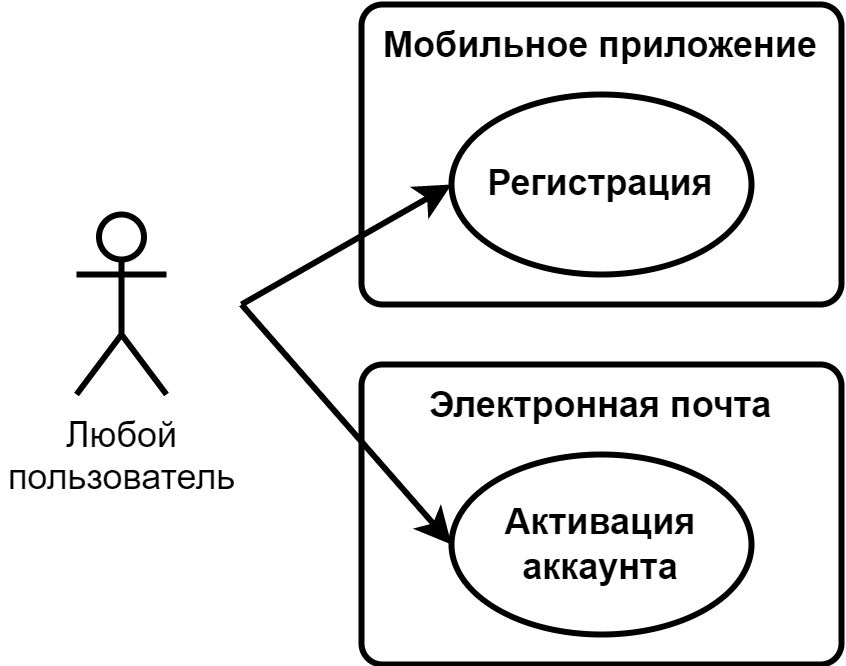
\includegraphics[width=18cm]
    {images/UML/UML_precedent_registration.png}

    \caption{Диаграмма прецедентов для регистрации}

    \label{fig:UML_precedent_registration}
\end{figure}

% = = = = = = = =

\subparagraph{Прецедент <<Заявка на смену электронной почты>>} \hspace{0pt}

\underline{Назначение}: смена электронной почты на новую.

\underline{Исполнители}: мобильный клиент.

\underline{Эндпоинт}: PATCH /api/v1/users/change-email.

\underline{Предусловие}: у пользователя есть токен доступа (access token).

\underline{Основной поток событий}: HTTP статус 200 (OK) - заявка отправлена на новую почту и предупреждение отправлено на старую почту.

\underline{Альтернативный поток событий}:

\begin{itemize}
    \item HTTP статус 401 (Unauthorized) - токен доступа просрочен;
    \item HTTP статус 401 (Unauthorized) - токен доступа не передан;
    \item HTTP статус 409 (Conflict) - новая почта совпадает с текущей;
    \item HTTP статус 429 (To Many Request) - слишком много запросов о смене электроной почты за не прошедшие 3 часа;
    \item HTTP статус 500 (Internal Server Error) - транзация не совершена, так как нет таблицы в БД (не сохранения запись о смене старой электронной почты на новую)
    \item HTTP статус 500 (Internal Server Error) - транзация не совершена, так как не отправлено письмо на новую и старую почту;
    \item HTTP статус 500 (Internal Server Error) - что-то пошло не так на сервере.
\end{itemize}

Диаграмма прецедентов изображены на рис.~\ref{fig:UML_precedent_change_email}.

% = = = = = = = =

\subparagraph{Прецедент <<Подтверждение смены электронной почты>>} \hspace{0pt}

\underline{Назначение}: подтверждение смены электронной почты.

\underline{Исполнители}: электронаая почта.

\underline{Эндпоинт}: GET /api/v1/users/change-email/:token/confirm.

\underline{Предусловие}: не прошло 3 часа.

\underline{Основной поток событий}: HTTP статус 200 (OK) - электронная почта изменена на новую.

\underline{Альтернативный поток событий}:

\begin{itemize}
    \item HTTP статус 404 (Not Found) - сылка не действительна, так как прошло 3 часа (токен просрочен);
    \item HTTP статус 404 (Not Found) - ссылка не действительна, так как токен подделан (токен не прошел валидацию);
    \item HTTP статус 404 (Not Found) - ссылка не действительна, так как токена не зарегистрирован в БД;
    \item HTTP статус 404 (Not Found) - ссылка не действительна, так как почта была сменена, либо заявка на смену почты была отклонена;
    \item HTTP статус 500 (Internal Server Error) - транзация не совернеша (заявка не отмечена закрытой, пользователю не поменял email на новый);
    \item HTTP статус 500 (Internal Server Error) - что-то пошло не так на сервере.
\end{itemize}

Диаграмма прецедентов изображены на рис.~\ref{fig:UML_precedent_change_email}.

% = = = = = = = =

\subparagraph{Прецедент <<Отмена заявки смены электронной почты>>} \hspace{0pt}

\underline{Назначение}: Отмена заявки смены электронной почты.

\underline{Исполнители}: электронная почта.

\underline{Эндпоинт}: GET /api/v1/users/change-email/:token/delete.

\underline{Предусловие}: не прошло 3 часа.

\underline{Основной поток событий}: HTTP статус 200 (OK) - заявка на смену электронной почты отменена.

\underline{Альтернативный поток событий}:

\begin{itemize}
    \item HTTP статус 404 (Not Found) - ссылка не действительна, так как прошло 3 часа (токен просрочен);
    \item HTTP статус 404 (Not Found) - ссылка не действительна, так как токен подделан (токен не прошел валидацию);
    \item HTTP статус 404 (Not Found) - ссылка не действительна, так как токен не зарегистрирован в БД;
    \item HTTP статус 404 (Not Found) - ссылка не действительна, так как почта была сменена, либо заявка на смену почты была отклонена;
    \item HTTP статус 500 (Internal Server Error) - нет таблицы в БД;
    \item HTTP статус 500 (Internal Server Error) - что-то пошло не так на сервере.
\end{itemize}

Диаграмма прецедентов изображены на рис.~\ref{fig:UML_precedent_change_email}.

% = = = = = = = =

\begin{figure}[!htb]
    \centering

    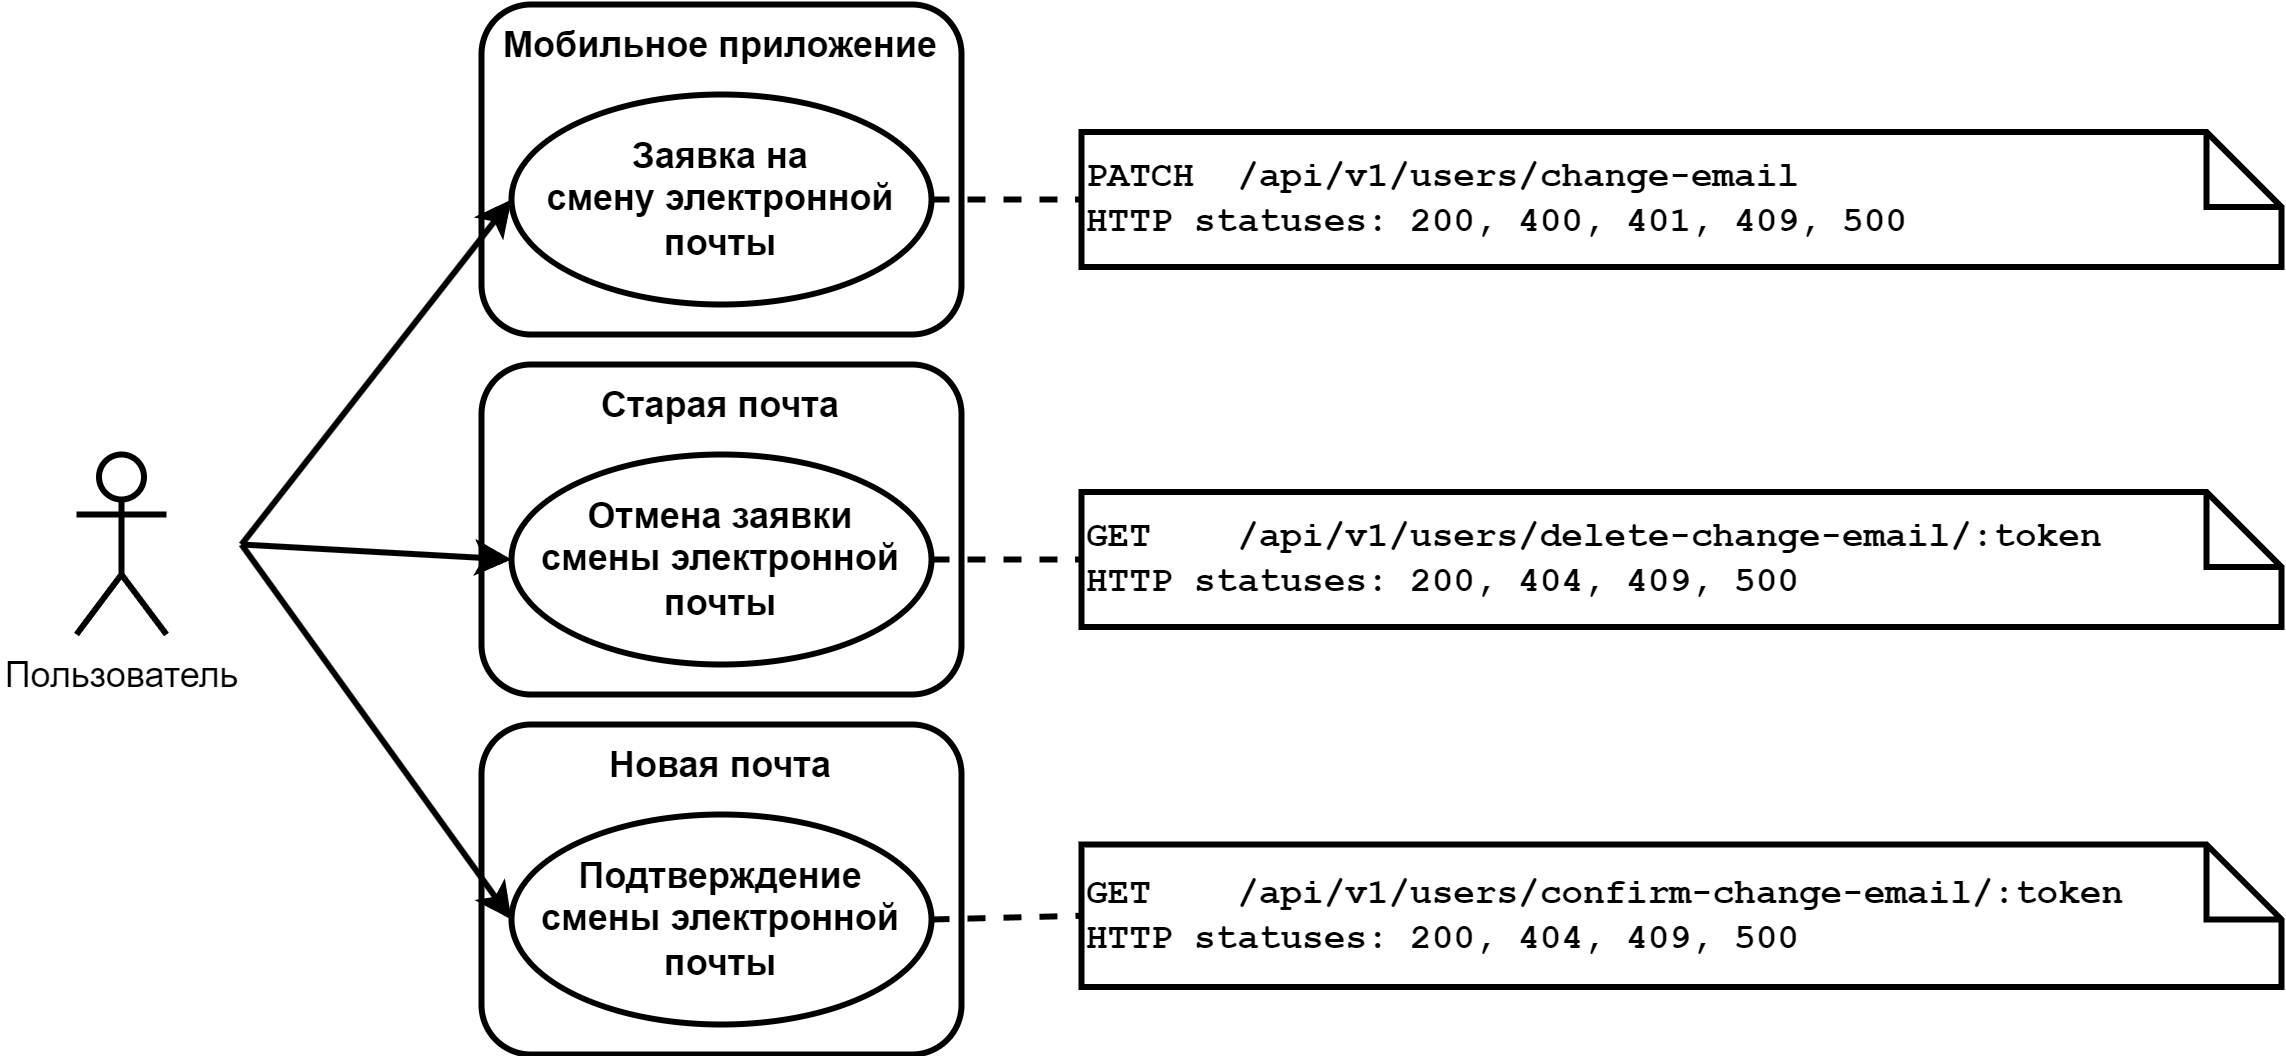
\includegraphics[width=18cm]
    {images/UML/UML_precedent_change_email.png}

    \caption{Диаграмма прецедентов для смены электронной почты}

    \label{fig:UML_precedent_change_email}
\end{figure}

% = = = = = = = =

\subparagraph{Прецедент <<Забыли пароль>>} \hspace{0pt}

\underline{Назначение}: на почту прийдет логин и новый сгенерированый пароль.

\underline{Исполнители}: мобильный клиент.

\underline{Эндпоинт}: POST /api/v1/users/forget-password.

\underline{Предусловие}: у пользователя есть токен доступа (access token).

\underline{Основной поток событий}: HTTP статус 200 (OK) - на электронную почту отправлен логин и новый сгенерированный пароль.

\underline{Альтернативный поток событий}:

\begin{itemize}
    \item HTTP статус 409 (Conflict) - пользователя с такой электронной почтой не существует;
    \item HTTP статус 500 (Internal Server Error) - транзация не совернеша, так как сгенерированный пароль не записался в БД;
    \item HTTP статус 500 (Internal Server Error) - транзация не совернеша, так как письмо с логином и паролем не отправлено на электронную почту;
    \item HTTP статус 500 (Internal Server Error) - что-то пошло не так на сервере.
\end{itemize}

Диаграмма прецедентов изображены на рис.~\ref{fig:UML_precedent_change_password}.

% = = = = = = = =

\subparagraph{Прецедент <<Смена пароля>>} \hspace{0pt}

\underline{Назначение}: смена пароля.

\underline{Исполнители}: мобильный клиент.

\underline{Эндпоинт}: PATCH /api/v1/users/change-password.

\underline{Предусловие}: у пользователя есть токен доступа (access token), пользователь указал верно старый пароль.

\underline{Основной поток событий}: HTTP статус 200 (OK) - пароль изменен. 

\underline{Альтернативный поток событий}:

\begin{itemize}
    \item HTTP статус 409 (Conflict) - не тот старый пароль;
    \item HTTP статус 500 (Internal Server Error) - транзация не совернеша, так как новый пароль не записан в БД;
    \item HTTP статус 500 (Internal Server Error) - транзация не совернеша, так как не удалось завершить все сессии;
    \item HTTP статус 500 (Internal Server Error) - что-то пошло не так на сервере.
\end{itemize}

Диаграмма прецедентов изображены на рис.~\ref{fig:UML_precedent_change_password}.

% = = = = = = = =

\begin{figure}[!htb]
    \centering

    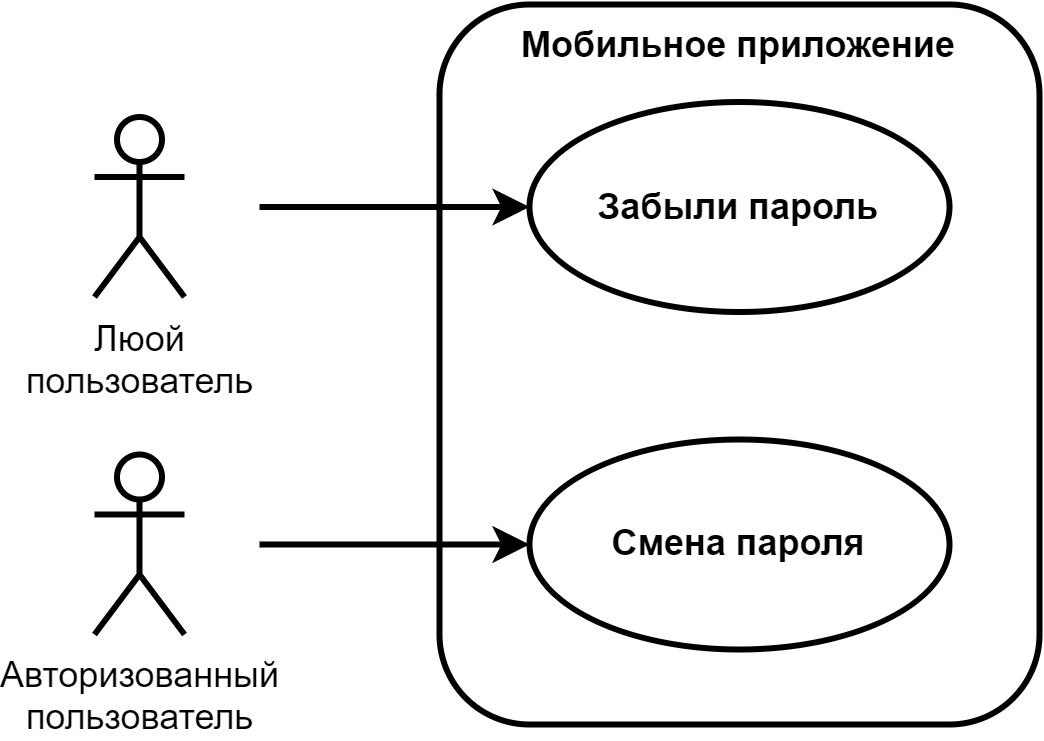
\includegraphics[width=18cm]
    {images/UML/UML_precedent_change_password.png}

    \caption{Диаграмма прецедентов для смены пароля}

    \label{fig:UML_precedent_change_password}
\end{figure}

% = = = = = = = =

\subparagraph{Прецедент <<Вход в аккаунт>>} \hspace{0pt}

\underline{Назначение}: ввойти в аккаунт.

\underline{Исполнители}: мобильный клиент.

\underline{Эндпоинт}: POST /api/v1/sessions.

\underline{Предусловие}: пользователь указал существующий логин и верный пароль.

\underline{Основной поток событий}: HTTP статус 201 (Created) - пользователь авторизовался (получил access и refresh токены). 

\underline{Альтернативный поток событий}:

\begin{itemize}
    \item HTTP статус 409 (Conflict) - нет пользователя с таким логином;
    \item HTTP статус 409 (Conflict) - не тот пароль.
    \item HTTP статус 500 (Internal Server Error) - что-то пошло не так на сервере.
\end{itemize}

Диаграмма прецедентов изображены на рис.~\ref{fig:UML_precedent_sessions}.

% = = = = = = = =

\subparagraph{Прецедент <<Получаем список сессий>>} \hspace{0pt}

\underline{Назначение}: получить список сессий.

\underline{Исполнители}: мобильный клиент.

\underline{Эндпоинт}: GET /api/v1/sessions.

\underline{Предусловие}: у пользователя есть токен доступа (access token).

\underline{Основной поток событий}: HTTP статус 200 (OK) - получили список ip и устройств. 

\underline{Альтернативный поток событий}: 

\begin{itemize}
    \item HTTP статус 401 (Unauthorized) - access токен просрочен;
    \item HTTP статус 401 (Unauthorized) - access токен не переда;
    \item HTTP статус 500 (Internal Server Error) - что-то пошло не так на сервере.
\end{itemize}

Диаграмма прецедентов изображены на рис.~\ref{fig:UML_precedent_sessions}.

% = = = = = = = =

\subparagraph{Прецедент <<Обновление токена доступа>>} \hspace{0pt}

\underline{Назначение}: обновить просроченый или потеряный токен доступа имея токено обновления.

\underline{Исполнители}: мобильный клиент.

\underline{Эндпоинт}: PATCH /api/v1/sessions.

\underline{Предусловие}: у пользователя есть токен обновления (refresh token).

\underline{Основной поток событий}: HTTP статус 200 (OK) - получили новый access токен. 

\underline{Альтернативный поток событий}:

\begin{itemize}
    \item HTTP статус 401 (Unauthorized) - refresh токен просрочен;
    \item HTTP статус 401 (Unauthorized) - refresh токен не передан;
    \item HTTP статус 500 (Internal Server Error) - что-то пошло не так на сервере.
\end{itemize}

Диаграмма прецедентов изображены на рис.~\ref{fig:UML_precedent_sessions}.

% = = = = = = = =

\subparagraph{Прецедент <<Завершение всех сессий>>} \hspace{0pt}

\underline{Назначение}: закрыть все сессии.

\underline{Исполнители}: мобильный клиент.

\underline{Эндпоинт}: DELETE /api/v1/sessions.

\underline{Предусловие}: у пользователя есть токен доступа (access token).

\underline{Основной поток событий}: HTTP статус 200 (OK) - закрыли все сессии. 

\underline{Альтернативный поток событий}:

\begin{itemize}
    \item HTTP статус 401 (Unauthorized) - access токен просрочен;
    \item HTTP статус 401 (Unauthorized) - access токен не передан;
    \item HTTP статус 500 (Internal Server Error) - что-то пошло не так на сервере.
\end{itemize}

Диаграмма прецедентов изображены на рис.~\ref{fig:UML_precedent_sessions}.

% = = = = = = = =

\subparagraph{Прецедент <<Завершение сессии по id>>} \hspace{0pt}

\underline{Назначение}: закрыть сессию по id.

\underline{Исполнители}: мобильный клиент.

\underline{Эндпоинт}: DELETE /api/v1/sessions/:id.

\underline{Предусловие}: у пользователя есть токен доступа (access token).

\underline{Основной поток событий}: HTTP статус 200 (OK) - закрыли сессию по id. 

\underline{Альтернативный поток событий}:

\begin{itemize}
    \item HTTP статус 401 (Unauthorized) - access токен просрочен;
    \item HTTP статус 401 (Unauthorized) - access токен не передан;
    \item HTTP статус 500 (Internal Server Error) - что-то пошло не так на сервере.
\end{itemize}

Диаграмма прецедентов изображены на рис.~\ref{fig:UML_precedent_sessions}.

% = = = = = = = =

\begin{figure}[!htb]
    \centering

    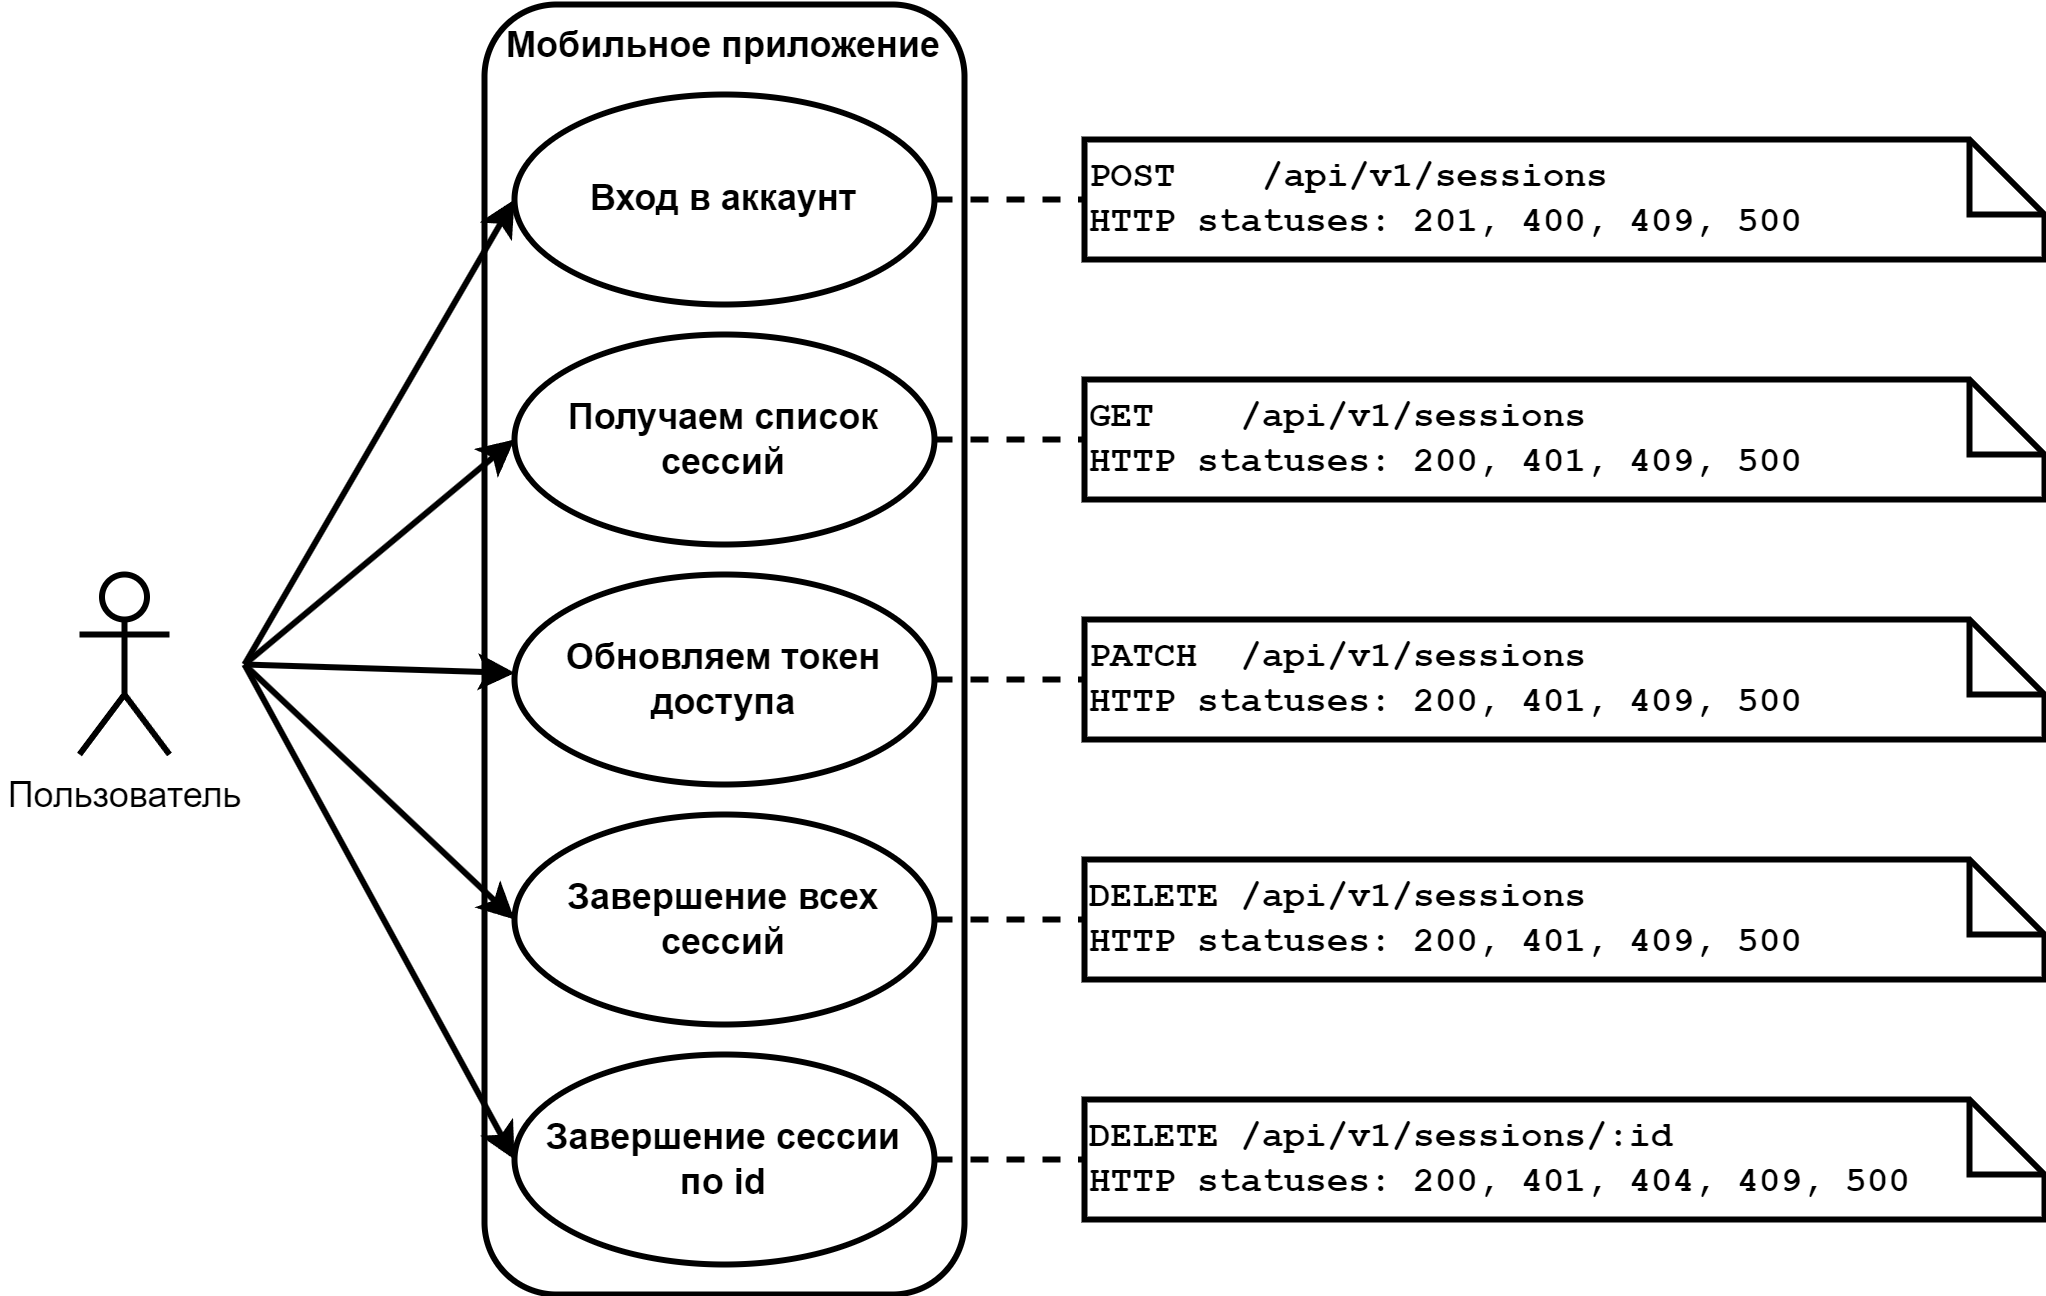
\includegraphics[width=18cm]
    {images/UML/UML_precedent_sessions.png}

    \caption{Диаграмма прецедентов для смены электронной почты}

    \label{fig:UML_precedent_sessions}
\end{figure}

% = = = = = = = =

\subparagraph{Прецедент <<Создание заявки товаров(-а)>>} \hspace{0pt}

\underline{Назначение}: создание заявка на отбор товаров(-а).

\underline{Исполнители}: мобильный клиент.

\underline{Эндпоинт}: POST /api/v1/order-items.

\underline{Предусловие}: у пользователя есть токен доступа (access token).

\underline{Основной поток событий}: HTTP статус 200 (OK) - пользователь оставил заявку на отбор товаров(-а). 

\underline{Альтернативный поток событий}:

\begin{itemize}
    \item HTTP статус 401 (Unauthorized) - пользователь не указал токен доступа;
    \item HTTP статус 401 (Unauthorized) - пользователь указал просроченый токен доступа (нет в БД);
    \item HTTP статус 500 (Internal Server Error) - что-то пошло не так на сервере.
\end{itemize}

Диаграмма прецедентов изображены на рис.~\ref{fig:UML_precedent_order_items}.

% = = = = = = = =

\subparagraph{Прецедент <<Просмотр списка заявок>>} \hspace{0pt}

\underline{Назначение}: просмотр список заявок.

\underline{Исполнители}: мобильный клиент.

\underline{Эндпоинт}: GET /api/v1/order-items.

\underline{Предусловие}: у пользователя есть токен доступа (access token).

\underline{Основной поток событий}: HTTP статус 200 (OK) - пользователь получил список заявок. 

\underline{Альтернативный поток событий}:

\begin{itemize}
    \item HTTP статус 401 (Unauthorized) - пользователь не указал токен доступа;
    \item HTTP статус 401 (Unauthorized) - пользователь указал просроченый токен доступа (нет в БД);
    \item HTTP статус 500 (Internal Server Error) - что-то пошло не так на сервере.
\end{itemize}

Диаграмма прецедентов изображены на рис.~\ref{fig:UML_precedent_order_items}.

% = = = = = = = =

\subparagraph{Прецедент <<Просмотр заявки по uuid>>} \hspace{0pt}

\underline{Назначение}: просмотр заказаных товаров.

\underline{Исполнители}: мобильный клиент.

\underline{Эндпоинт}: GET /api/v1/order-items/:uuid.

\underline{Предусловие}: у пользователя есть токен доступа (access token).

\underline{Основной поток событий}: HTTP статус 200 (OK) - пользователь получил список товаров в заявке. 

\underline{Альтернативный поток событий}:

\begin{itemize}
    \item HTTP статус 401 (Unauthorized) - пользователь не указал токен доступа;
    \item HTTP статус 401 (Unauthorized) - пользователь указал просроченый токен доступа (нет в БД);
    \item HTTP статус 404 (Not Found) - такой заявки не существует;
    \item HTTP статус 500 (Internal Server Error) - что-то пошло не так на сервере.
\end{itemize}

Диаграмма прецедентов изображены на рис.~\ref{fig:UML_precedent_order_items}.

% = = = = = = = =

\subparagraph{Прецедент <<Отмена заявки по uuid>>} \hspace{0pt}

\underline{Назначение}: отмена заявки.

\underline{Исполнители}: мобильный клиент.

\underline{Эндпоинт}: DELETE /api/v1/order-items/:uuid.

\underline{Предусловие}: у пользователя есть токен доступа (access token).

\underline{Основной поток событий}: HTTP статус 200 (OK) - пользователь отменил заявку. 

\underline{Альтернативный поток событий}:

\begin{itemize}
    \item HTTP статус 401 (Unauthorized) - пользователь не указал токен доступа;
    \item HTTP статус 401 (Unauthorized) - пользователь указал просроченый токен доступа (нет в БД);
    \item HTTP статус 404 (Not Found) - такой заявки не существует;
    \item HTTP статус 500 (Internal Server Error) - что-то пошло не так на сервере.
\end{itemize}

Диаграмма прецедентов изображены на рис.~\ref{fig:UML_precedent_order_items}.

% = = = = = = = =

\subparagraph{Прецедент <<Просмотр статуса отбора товаров(-а)>>} \hspace{0pt}

\underline{Назначение}: просмотреть статус отбора товаров(-а).

\underline{Исполнители}: мобильный клиент, браузер.

\underline{Эндпоинт}: GET /api/v1/order-items/:uuid/status.

\underline{Предусловие}: uuid заявки найден в БД.

\underline{Основной поток событий}: HTTP статус 200 (OK) - пользователь получил список статусов о состоянии отбора товаров(-а). 

\underline{Альтернативный поток событий}:

\begin{itemize}
    \item HTTP статус 404 (Not Found) - заявка не найдена;
    \item HTTP статус 500 (Internal Server Error) - что-то пошло не так на сервере.
\end{itemize}

Диаграмма прецедентов изображены на рис.~\ref{fig:UML_precedent_order_items}.

% = = = = = = = =

\begin{figure}[!htb]
    \centering

    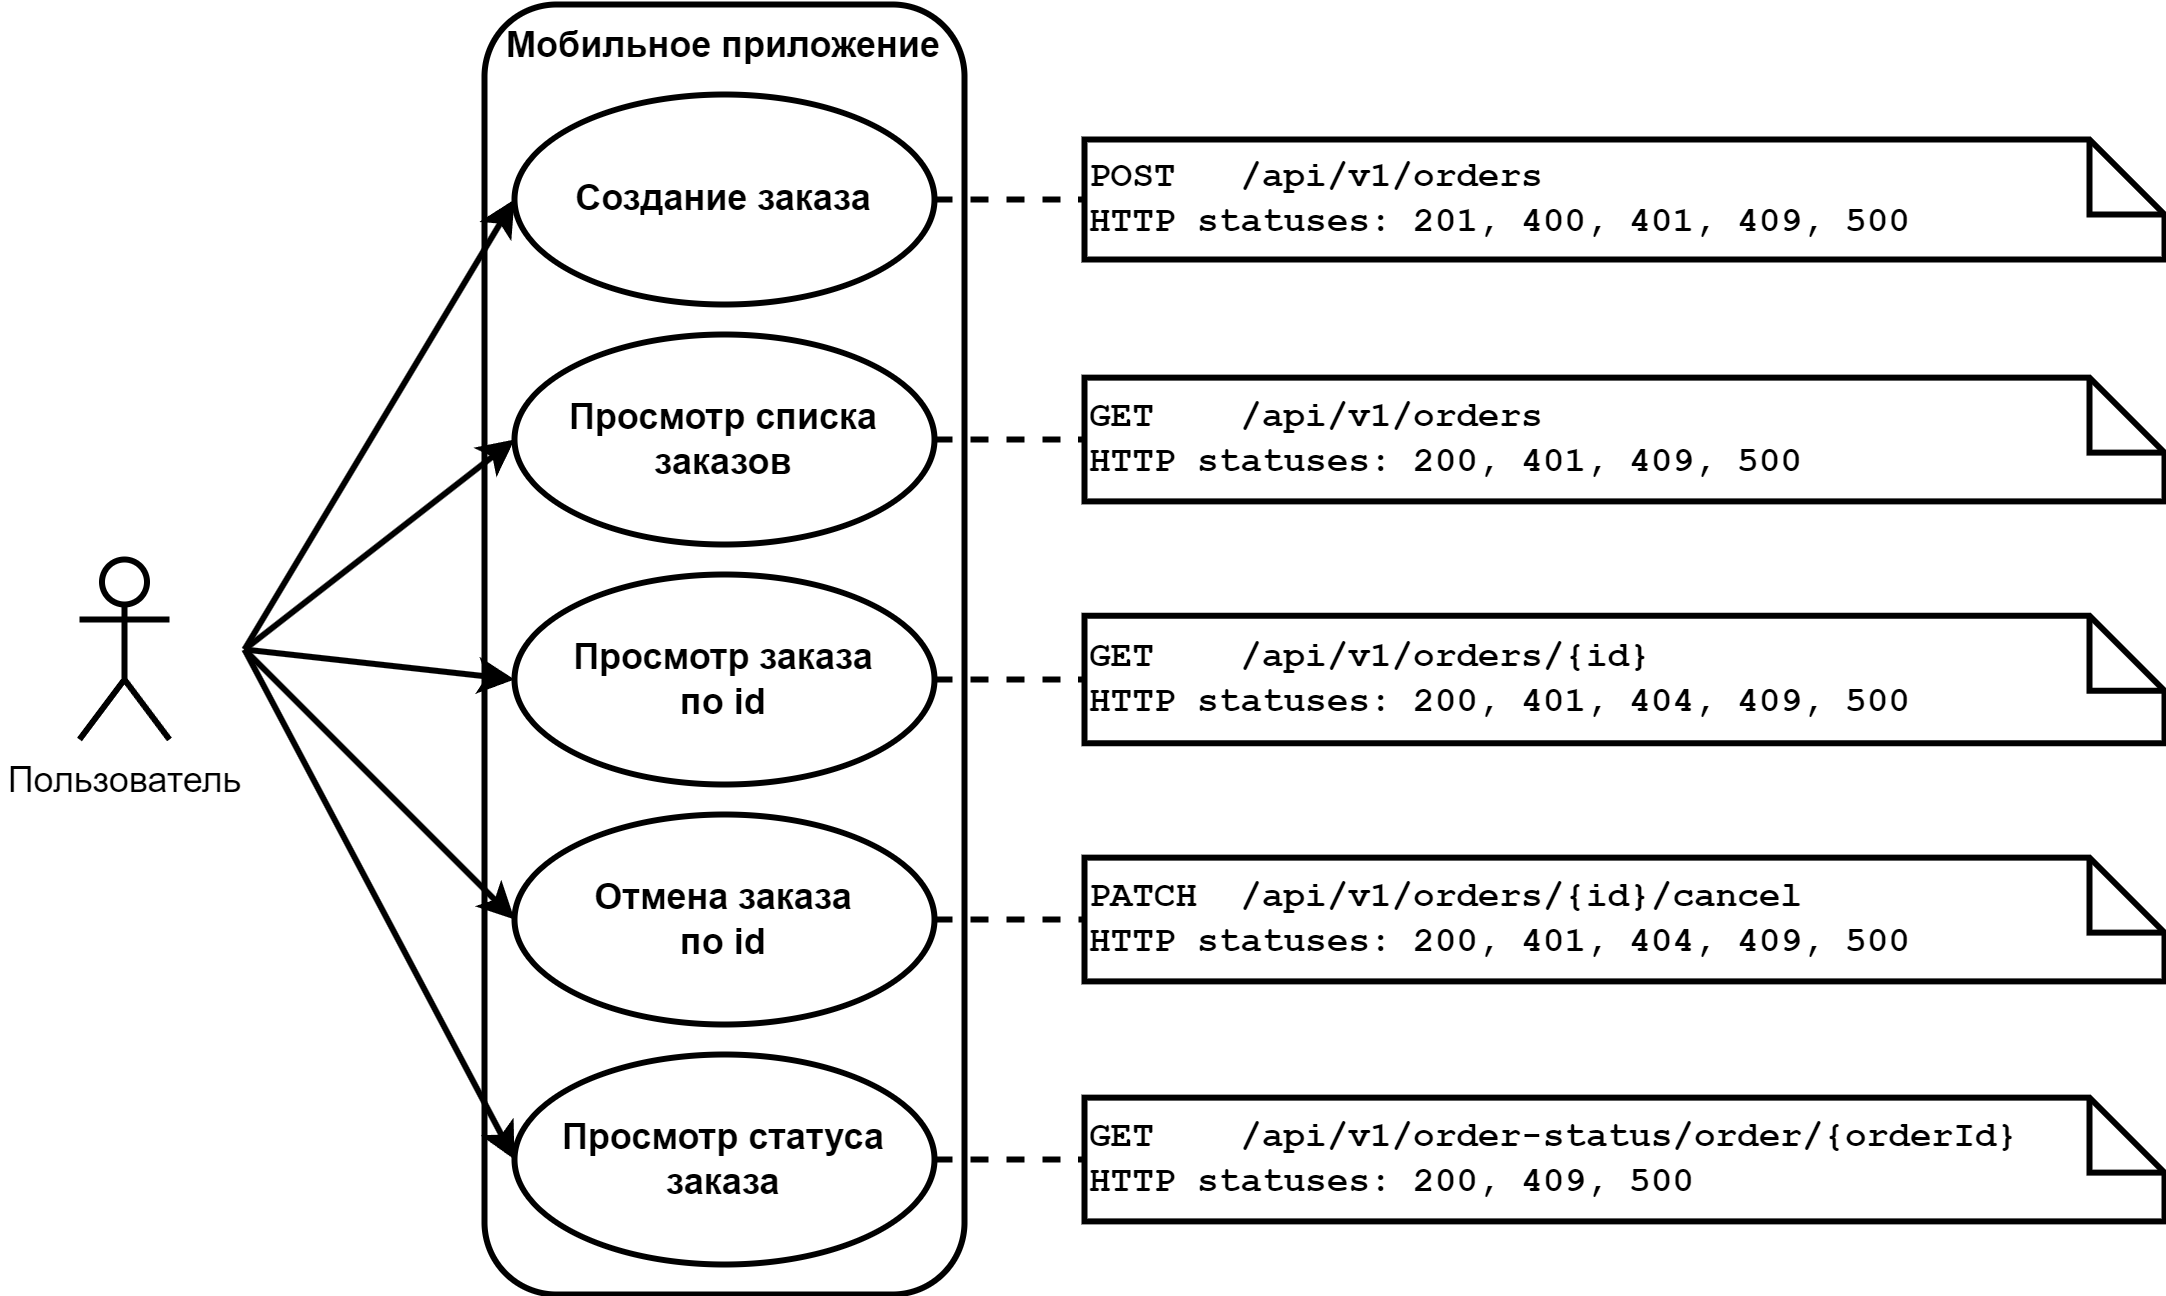
\includegraphics[width=18cm]
    {images/UML/UML_precedent_order_items.png}

    \caption{Диаграмма прецедентов для заявки отбора товаров}

    \label{fig:UML_precedent_order_items}
\end{figure}

% = = = = = = = =

\subparagraph{Прецедент <<Создание номенклатуры>>} \hspace{0pt}

\underline{Назначение}: запись номенклатуры в БД.

\underline{Исполнители}: администратор, браузер.

\underline{Эндпоинт}: POST /api/v1/items.

\underline{Предусловие}: у пользователя есть токен доступа и роль admin.

\underline{Основной поток событий}: HTTP статус 201 (Created) - администратор создал номенклатуру в БД. 

\underline{Альтернативный поток событий}:
HTTP статус 500 (Internal Server Error) - что-то пошло не так на сервере.

Диаграмма прецедентов изображены на рис.~\ref{fig:UML_precedent_items}.

% = = = = = = = =

\subparagraph{Прецедент <<Просмотр списка номенклатуры>>} \hspace{0pt}

\underline{Назначение}: просмотр списка номенклатуры.

\underline{Исполнители}: мобильный клиент, браузер.

\underline{Эндпоинт}: GET /api/v1/items.

% \underline{Предусловие}: 

\underline{Основной поток событий}: HTTP статус 200 (OK) - пользователь получил список номенклатуры. 

\underline{Альтернативный поток событий}:
HTTP статус 500 (Internal Server Error) - что-то пошло не так на сервере.

Диаграмма прецедентов изображены на рис.~\ref{fig:UML_precedent_items}.

% = = = = = = = =

\subparagraph{Прецедент <<Просмотр номенклатуры по uuid>>} \hspace{0pt}

\underline{Назначение}: просмотр определённой номенклатуры.

\underline{Исполнители}: мобильный клиент, браузер.

\underline{Эндпоинт}: GET /api/v1/items/:uuid.

% \underline{Предусловие}: 

\underline{Основной поток событий}: HTTP статус 200 (OK) - пользователь получил данные номенклатуры по uuid. 

\underline{Альтернативный поток событий}:

\begin{itemize}
    \item HTTP статус 404 (Not Found) - данные о номенклатуре по uuid не найдены;
    \item HTTP статус 500 (Internal Server Error) - что-то пошло не так на сервере.
\end{itemize}

Диаграмма прецедентов изображены на рис.~\ref{fig:UML_precedent_items}.

% = = = = = = = =

\subparagraph{Прецедент <<Обновление номенклатуры по uuid>>} \hspace{0pt}

\underline{Назначение}: обновить данные о номенклатуре по uuid.

\underline{Исполнители}: администратор, браузер.

\underline{Эндпоинт}: PATCH /api/v1/items/:uuid.

\underline{Предусловие}: у пользователя есть токен доступа и роль admin.

\underline{Основной поток событий}: HTTP статус 200 (OK) - администратор обновил данные о номенклатуре по uuid. 

\underline{Альтернативный поток событий}:

\begin{itemize}
    \item HTTP статус 404 (Not Found) - данные о номенклатуре по uuid не найдены;
    \item HTTP статус 500 (Internal Server Error) - что-то пошло не так на сервере.
\end{itemize}

Диаграмма прецедентов изображены на рис.~\ref{fig:UML_precedent_items}.

% = = = = = = = =

\subparagraph{Прецедент <<Удаление номенклатуры по uuid>>} \hspace{0pt}

\underline{Назначение}: удалить данные о номенклатуре по uuid.

\underline{Исполнители}: администратор, браузер.

\underline{Эндпоинт}: DELETE /api/v1/items/:uuid.

\underline{Предусловие}: у пользователя есть токен доступа и роль admin.

\underline{Основной поток событий}: HTTP статус 200 (OK) - администратор обновил данные о номенклатуре по uuid. 

\underline{Альтернативный поток событий}:

\begin{itemize}
    \item HTTP статус 404 (Not Found) - данные о номенклатуре по uuid не найдены;
    \item HTTP статус 500 (Internal Server Error) - что-то пошло не так на сервере.
\end{itemize}

Диаграмма прецедентов изображены на рис.~\ref{fig:UML_precedent_items}.

% = = = = = = = =

\begin{figure}[!htb]
    \centering

    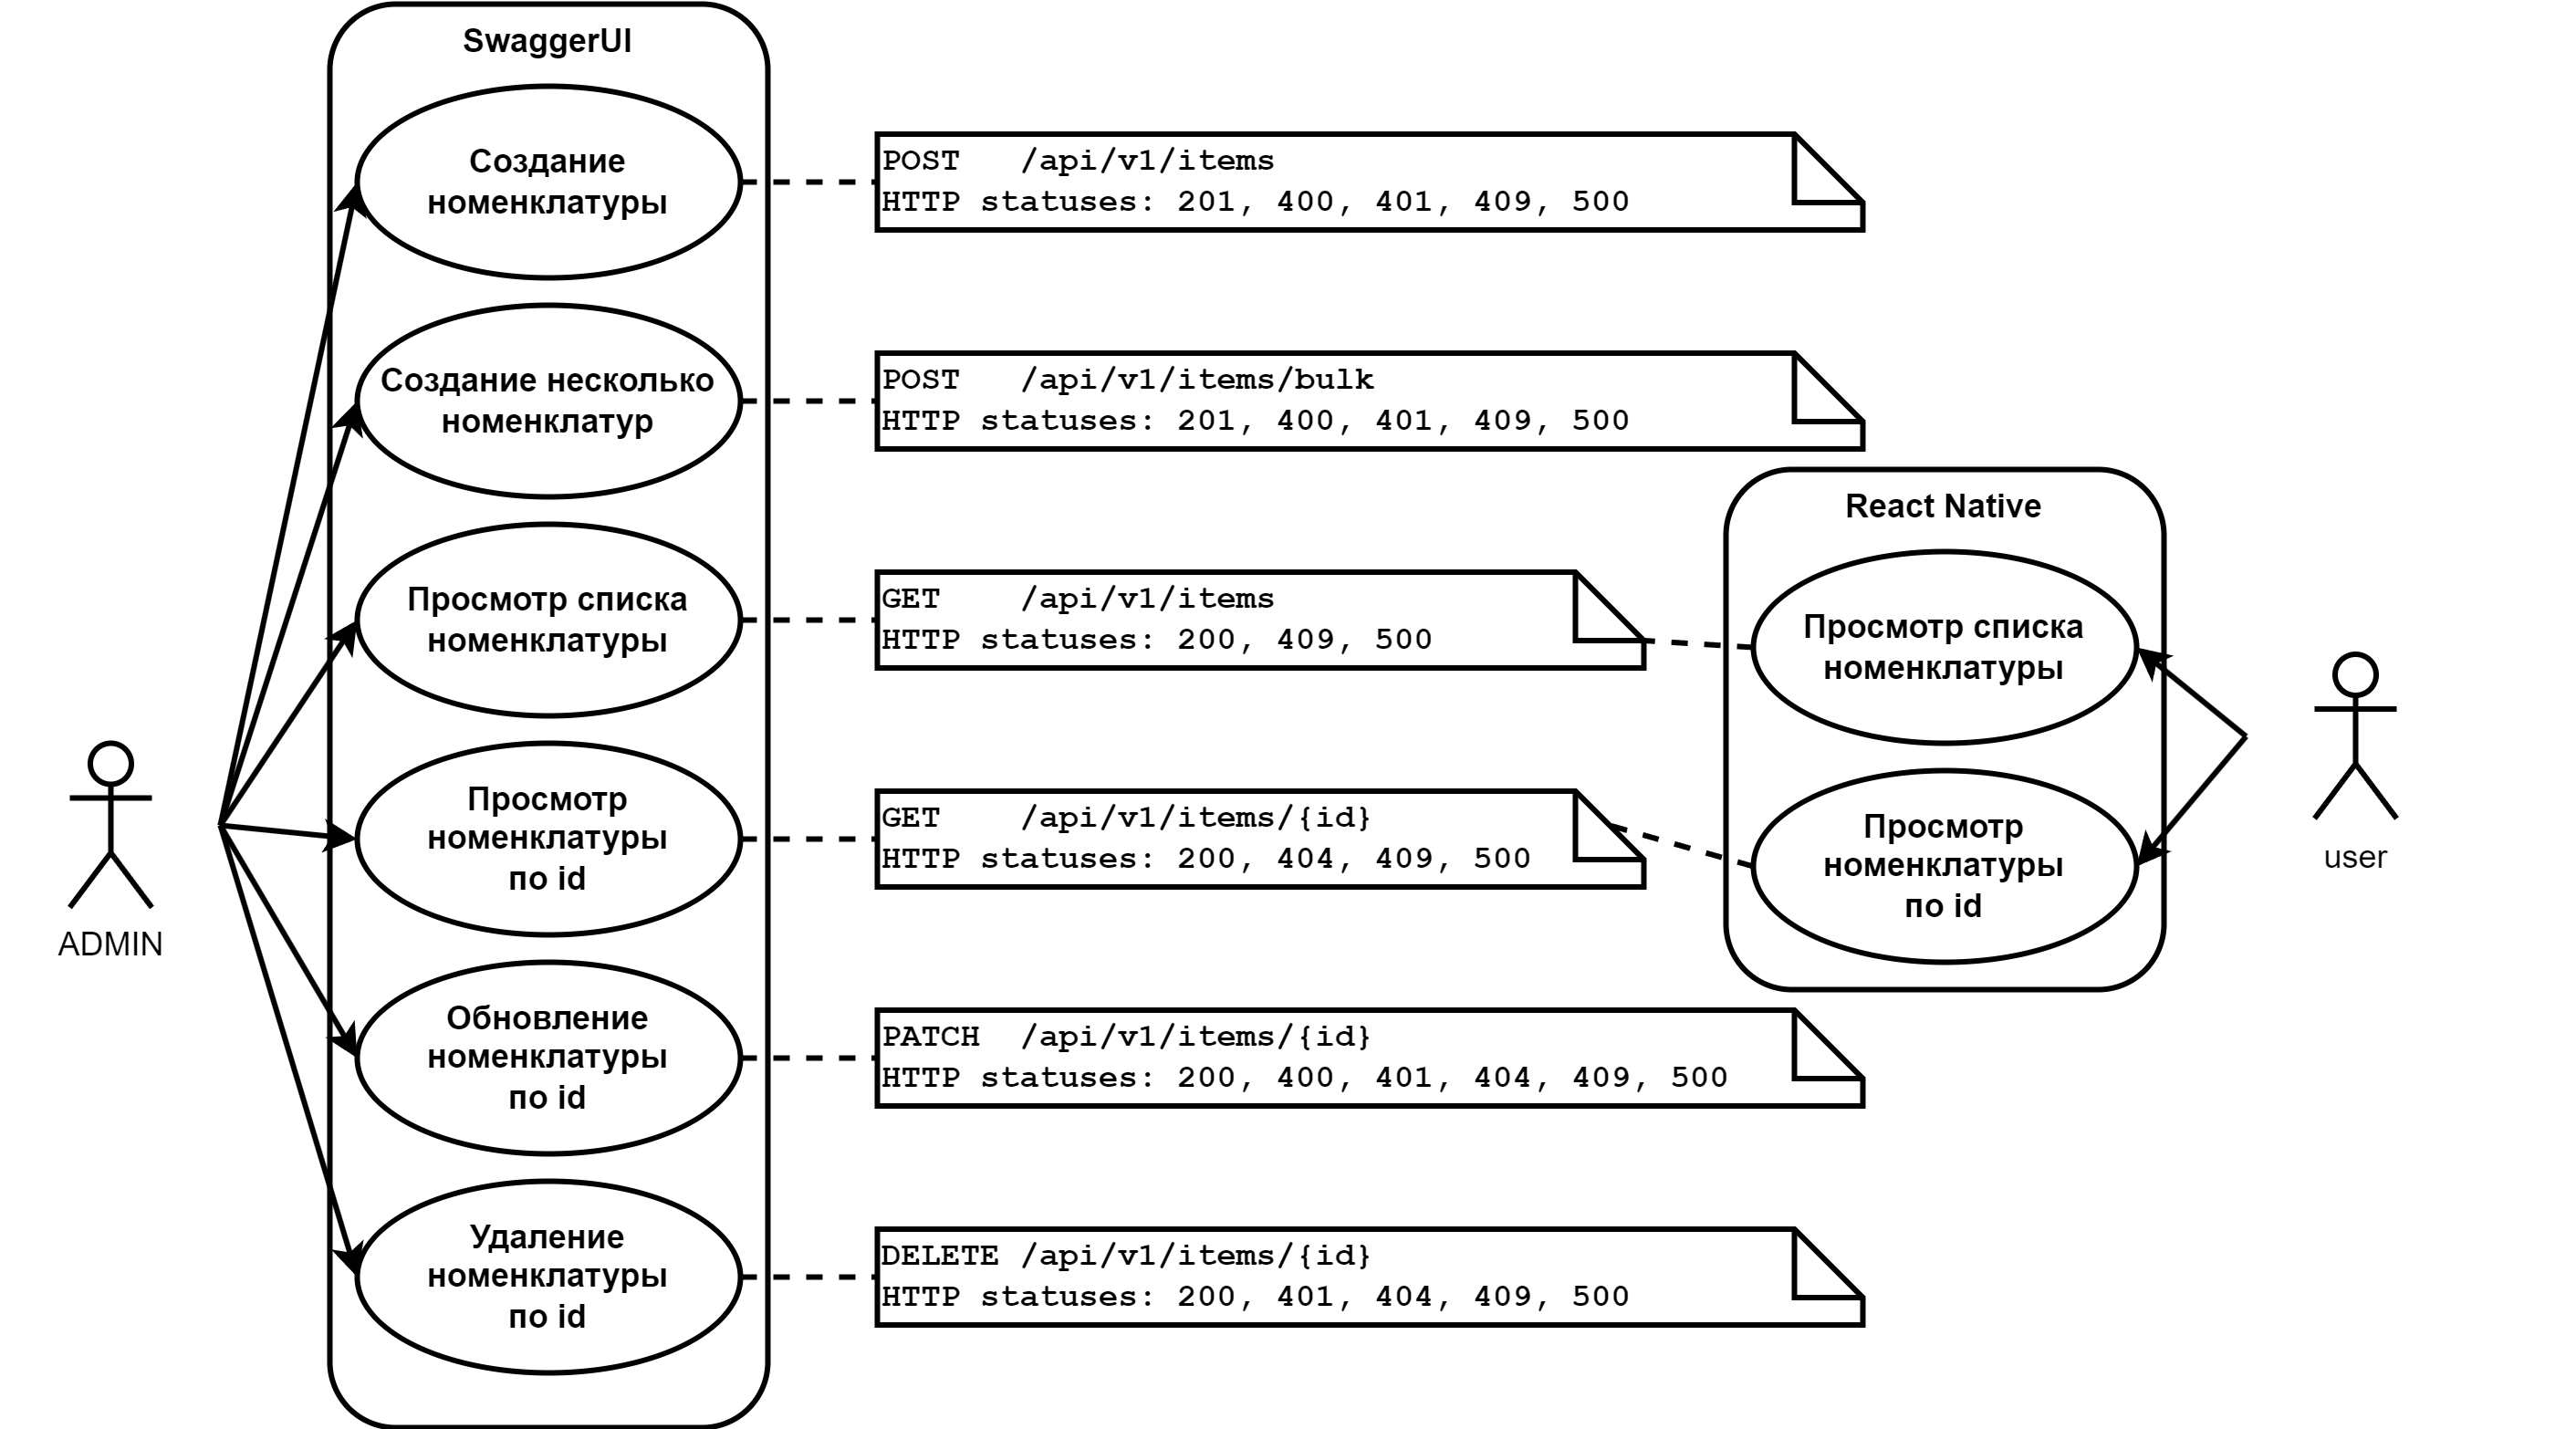
\includegraphics[width=17cm]
    {images/UML/UML_precedent_items.png}

    \caption{Диаграмма прецедентов для манипуляции с номенклутурой}

    \label{fig:UML_precedent_items}
\end{figure}

% = = = = = = = =

\subparagraph{Прецедент <<Создание категории номенклатуры>>} \hspace{0pt}

\underline{Назначение}: записать категорию номенклатуры в БД.

\underline{Исполнители}: администратор, браузер.

\underline{Эндпоинт}: POST /api/v1/item-categories.

\underline{Предусловие}: у пользователя есть токен доступа и роль admin.

\underline{Основной поток событий}: HTTP статус 201 (Created) - администратор создал категорию номенклатуры в БД. 

\underline{Альтернативный поток событий}:
HTTP статус 500 (Internal Server Error) - что-то пошло не так на сервере.

Диаграмма прецедентов изображены на рис.~\ref{fig:UML_precedent_item_categories}.

% = = = = = = = =

\subparagraph{Прецедент <<Просмотр списка категорий номенклатуры>>} \hspace{0pt}

\underline{Назначение}: просмотр списка категорий номенклатуры.

\underline{Исполнители}: мобильный клиент, браузер.

\underline{Эндпоинт}: GET /api/v1/item-categories.

% \underline{Предусловие}: 

\underline{Основной поток событий}: HTTP статус 200 (OK) - пользователь получил список номенклатуры. 

\underline{Альтернативный поток событий}:
HTTP статус 500 (Internal Server Error) - что-то пошло не так на сервере.

Диаграмма прецедентов изображены на рис.~\ref{fig:UML_precedent_item_categories}.

% = = = = = = = =

\subparagraph{Прецедент <<Просмотр категории номенклатуры по id>>} \hspace{0pt}

\underline{Назначение}: просмотр определённой номенклатуры.

\underline{Исполнители}: мобильный клиент, браузер.

\underline{Эндпоинт}: GET /api/v1/item-categories/:id.

% \underline{Предусловие}: 

\underline{Основной поток событий}: HTTP статус 200 (OK) - пользователь получил данные категории номенклатуры по id. 

\underline{Альтернативный поток событий}:

\begin{itemize}
    \item HTTP статус 404 (Not Found) - данные о категории номенклатуры по указанному id не найдены;
    \item HTTP статус 500 (Internal Server Error) - что-то пошло не так на сервере.
\end{itemize}

Диаграмма прецедентов изображены на рис.~\ref{fig:UML_precedent_item_categories}.

% = = = = = = = =

\subparagraph{Прецедент <<Обновление категории номенклатуры по id>>} \hspace{0pt}

\underline{Назначение}: обновить данные о номенклатуре по id.

\underline{Исполнители}: администратор, браузер.

\underline{Эндпоинт}: PATCH /api/v1/item-categories/:id.

\underline{Предусловие}: у пользователя есть токен доступа и роль admin.

\underline{Основной поток событий}: HTTP статус 200 (OK) - администратор обновил данные о категории номенклатуры по id. 

\underline{Альтернативный поток событий}:

\begin{itemize}
    \item HTTP статус 404 (Not Found) - данные о категории номенклатура по id не найдены;
    \item HTTP статус 500 (Internal Server Error) - что-то пошло не так на сервере.
\end{itemize}

Диаграмма прецедентов изображены на рис.~\ref{fig:UML_precedent_item_categories}.

% = = = = = = = =

\subparagraph{Прецедент <<Удаление категории номенклатуры по id>>} \hspace{0pt}

\underline{Назначение}: удалить данные о категории номенклатуры по id.

\underline{Исполнители}: администратор, браузер.

\underline{Эндпоинт}: DELETE /api/v1/item-categories/:id.

\underline{Предусловие}: у пользователя есть токен доступа и роль admin.

\underline{Основной поток событий}: HTTP статус 200 (OK) - администратор обновил данные о номенклатуре по uuid. 

\underline{Альтернативный поток событий}:

\begin{itemize}
    \item HTTP статус 404 (Not Found) - данные о категории номенклатуры по id не найдены;
    \item HTTP статус 500 (Internal Server Error) - что-то пошло не так на сервере.
\end{itemize}

Диаграмма прецедентов изображены на рис.~\ref{fig:UML_precedent_item_categories}.

% = = = = = = = =

\begin{figure}[!htb]
    \centering

    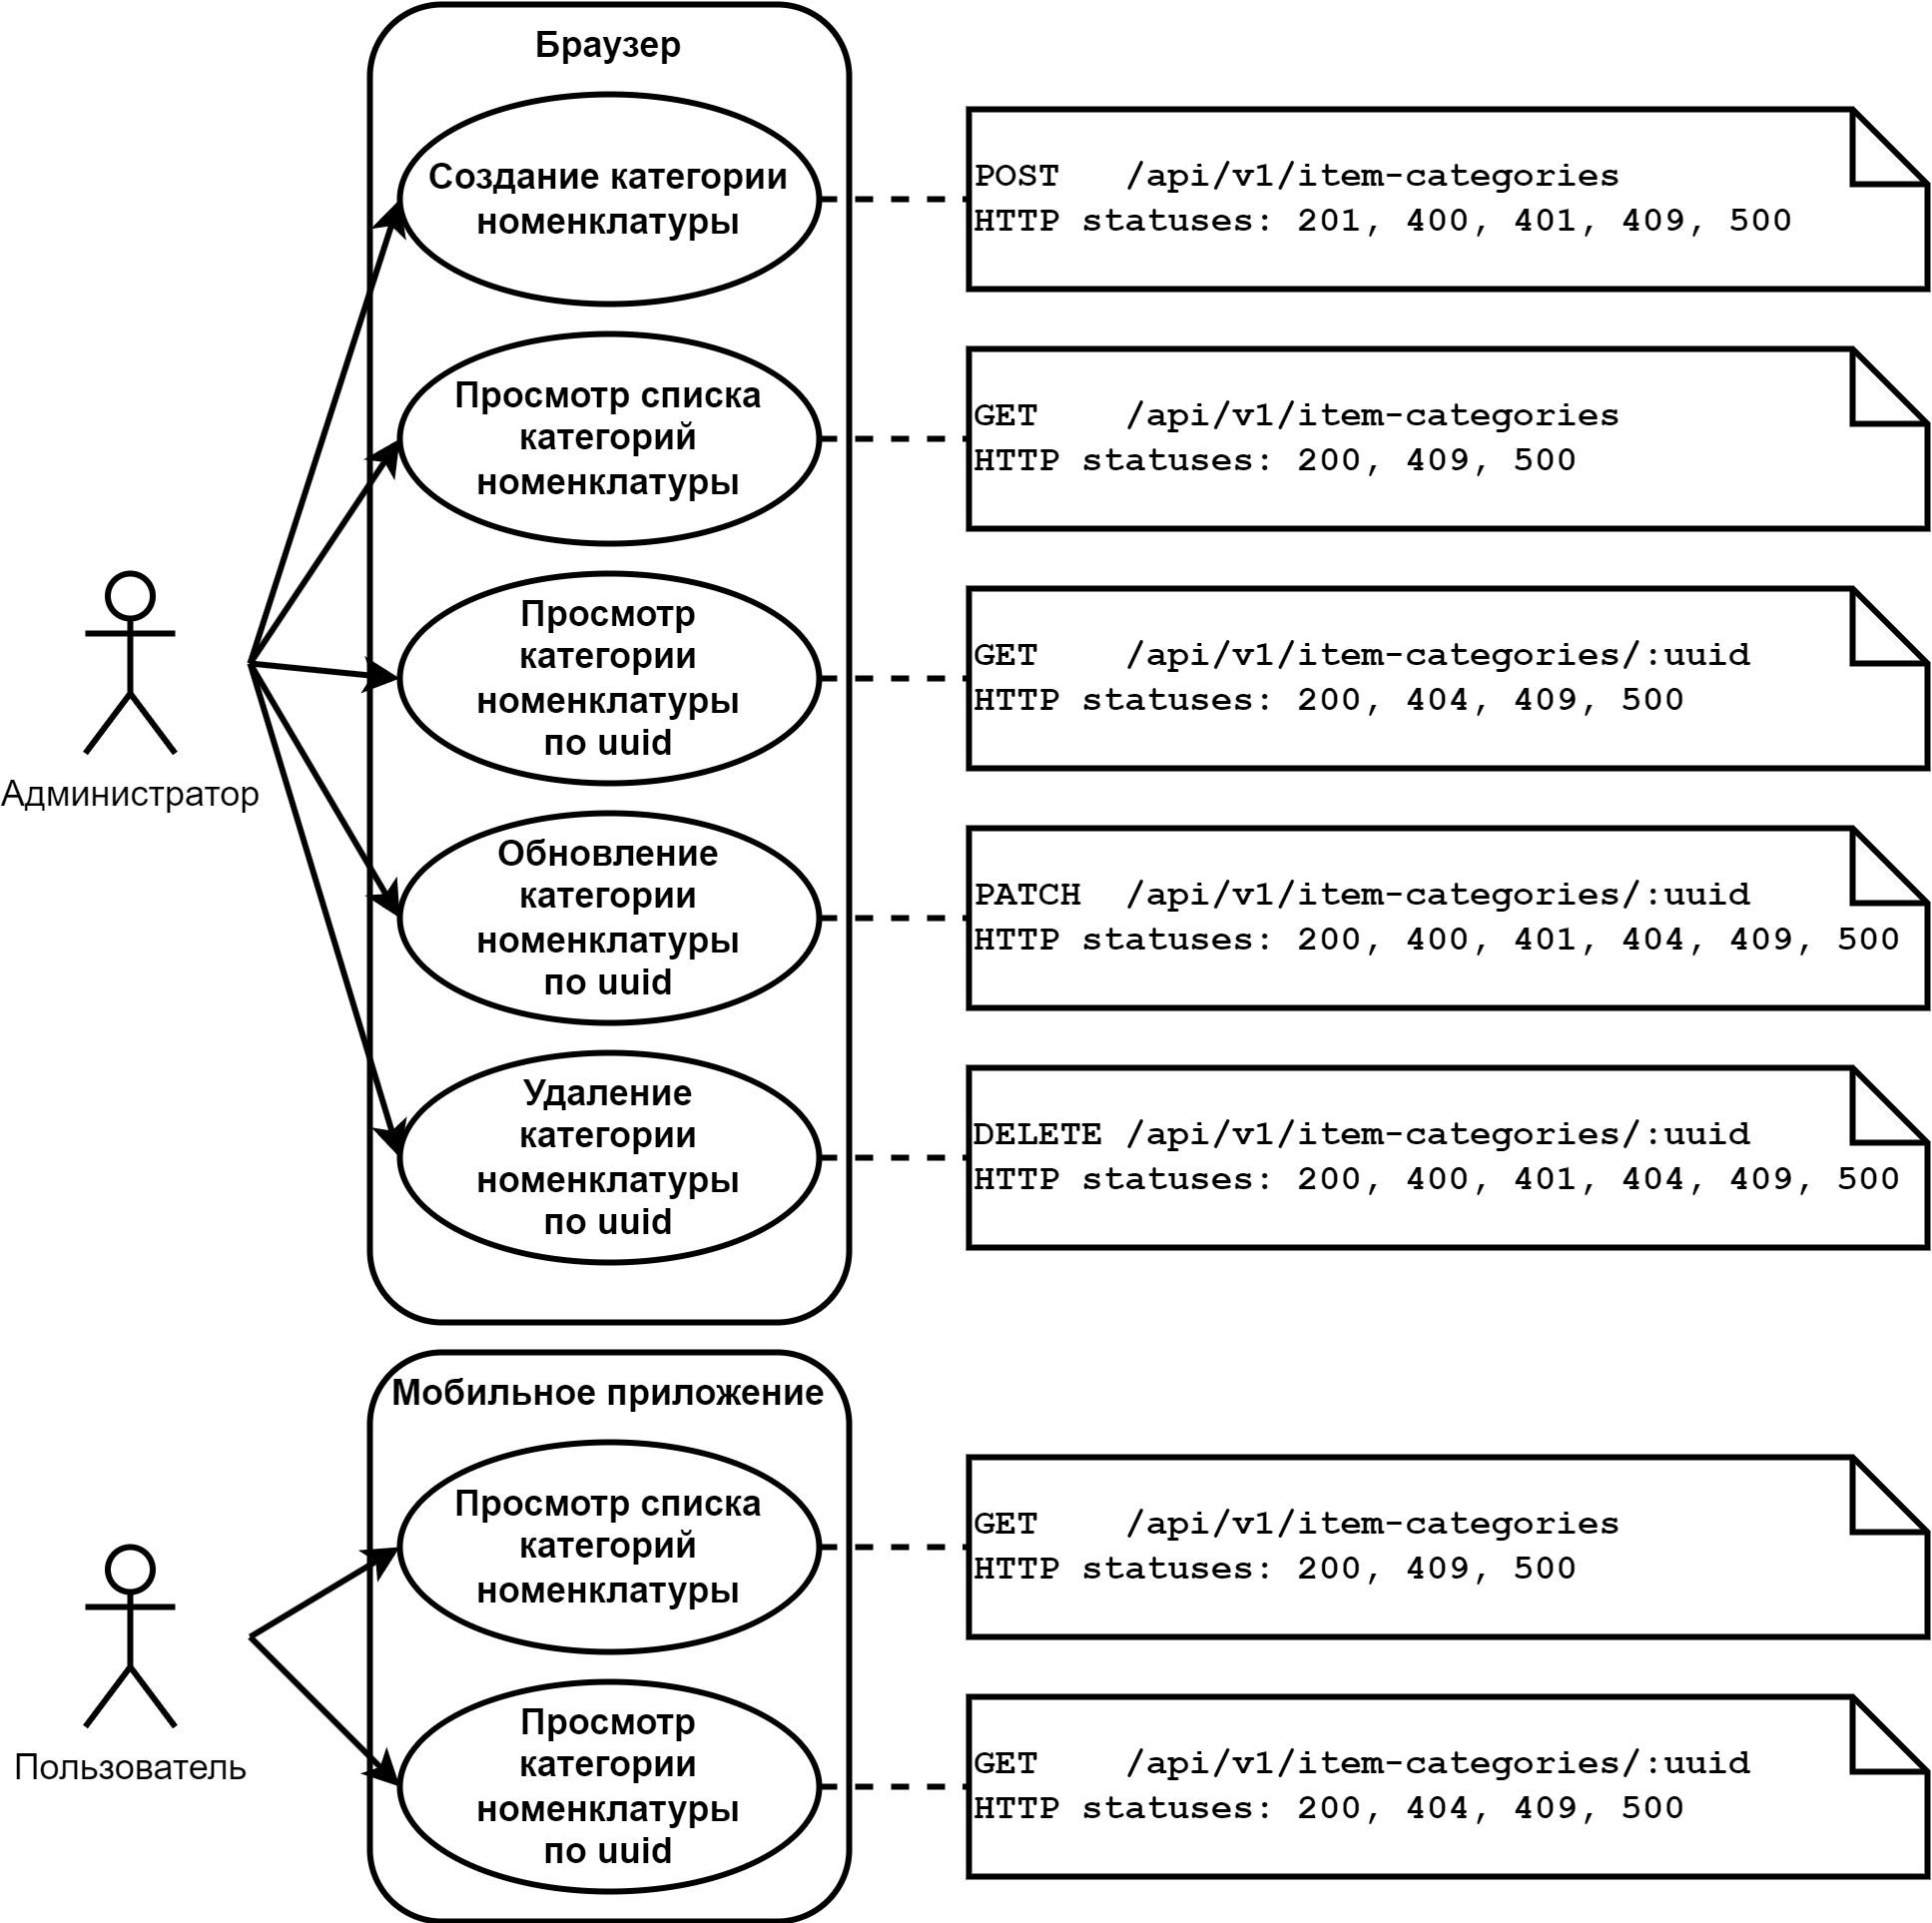
\includegraphics[width=15cm]
    {images/UML/UML_precedent_item_categories.png}

    \caption{Диаграмма прецедентов для манипуляции с категориями номенклатуры}

    \label{fig:UML_precedent_item_categories}
\end{figure}

% = = = = = = = =

\subparagraph{Прецедент <<Создание помощника (контакта рабочего)>>} \hspace{0pt}

\underline{Назначение}: создать контакт работника, который будет доступен в интернете, чтобы с ним связаться.

\underline{Исполнители}: администратор, браузер.

\underline{Эндпоинт}: POST /api/v1/helpers.

\underline{Предусловие}: у пользователя есть токен доступа и роль admin.

\underline{Основной поток событий}: HTTP статус 201 (Created) - администратор создал помощника в БД. 

\underline{Альтернативный поток событий}:
HTTP статус 500 (Internal Server Error) - что-то пошло не так на сервере.

Диаграмма прецедентов изображены на рис.~\ref{fig:UML_precedent_helpres}.

% = = = = = = = =

\subparagraph{Прецедент <<Просмотр списка помощников>>} \hspace{0pt}

\underline{Назначение}: просмотр списка помощников.

\underline{Исполнители}: мобильный клиент, браузер.

\underline{Эндпоинт}: GET /api/v1/helpers.

% \underline{Предусловие}: 

\underline{Основной поток событий}: HTTP статус 200 (OK) - пользователь получил список помощников. 

\underline{Альтернативный поток событий}:
HTTP статус 500 (Internal Server Error) - что-то пошло не так на сервере.

Диаграмма прецедентов изображены на рис.~\ref{fig:UML_precedent_helpres}.

% = = = = = = = =

\subparagraph{Прецедент <<Просмотр помощника по id>>} \hspace{0pt}

\underline{Назначение}: просмотр данных определённого помощника.

\underline{Исполнители}: мобильный клиент, браузер.

\underline{Эндпоинт}: GET /api/v1/helpers/:id.

% \underline{Предусловие}: 

\underline{Основной поток событий}: HTTP статус 200 (OK) - пользователь получил данные помощника по id. 

\underline{Альтернативный поток событий}:

\begin{itemize}
    \item HTTP статус 404 (Not Found) - данные о помощнике по указанному id не найдены;
    \item HTTP статус 500 (Internal Server Error) - что-то пошло не так на сервере.
\end{itemize}

Диаграмма прецедентов изображены на рис.~\ref{fig:UML_precedent_helpres}.

% = = = = = = = =

\subparagraph{Прецедент <<Обновление помощника по id>>} \hspace{0pt}

\underline{Назначение}: обновить данные о помощнике по id.

\underline{Исполнители}: администратор, браузер.

\underline{Эндпоинт}: PATCH /api/v1/helper/:id.

\underline{Предусловие}: у пользователя есть токен доступа и роль admin.

\underline{Основной поток событий}: HTTP статус 200 (OK) - администратор обновил данные о помощнике по id. 

\underline{Альтернативный поток событий}:

\begin{itemize}
    \item HTTP статус 404 (Not Found) - данные о помощнике по id не найдены;
    \item HTTP статус 500 (Internal Server Error) - что-то пошло не так на сервере.
\end{itemize}

Диаграмма прецедентов изображены на рис.~\ref{fig:UML_precedent_helpres}.

% = = = = = = = =

\subparagraph{Прецедент <<Удаление помощника по id>>} \hspace{0pt}

\underline{Назначение}: удалить данные о помощнике по id.

\underline{Исполнители}: администратор, браузер.

\underline{Эндпоинт}: DELETE /api/v1/item-categories/:id.

\underline{Предусловие}: у пользователя есть токен доступа и роль admin.

\underline{Основной поток событий}: HTTP статус 200 (OK) - администратор удалил данные о помощнике по id. 

\underline{Альтернативный поток событий}:

\begin{itemize}
    \item HTTP статус 404 (Not Found) - данные о помощнике по id не найдены;
    \item HTTP статус 500 (Internal Server Error) - что-то пошло не так на сервере.
\end{itemize}

Диаграмма прецедентов изображены на рис.~\ref{fig:UML_precedent_helpres}.

% = = = = = = = =

\begin{figure}[!p]
    \centering

    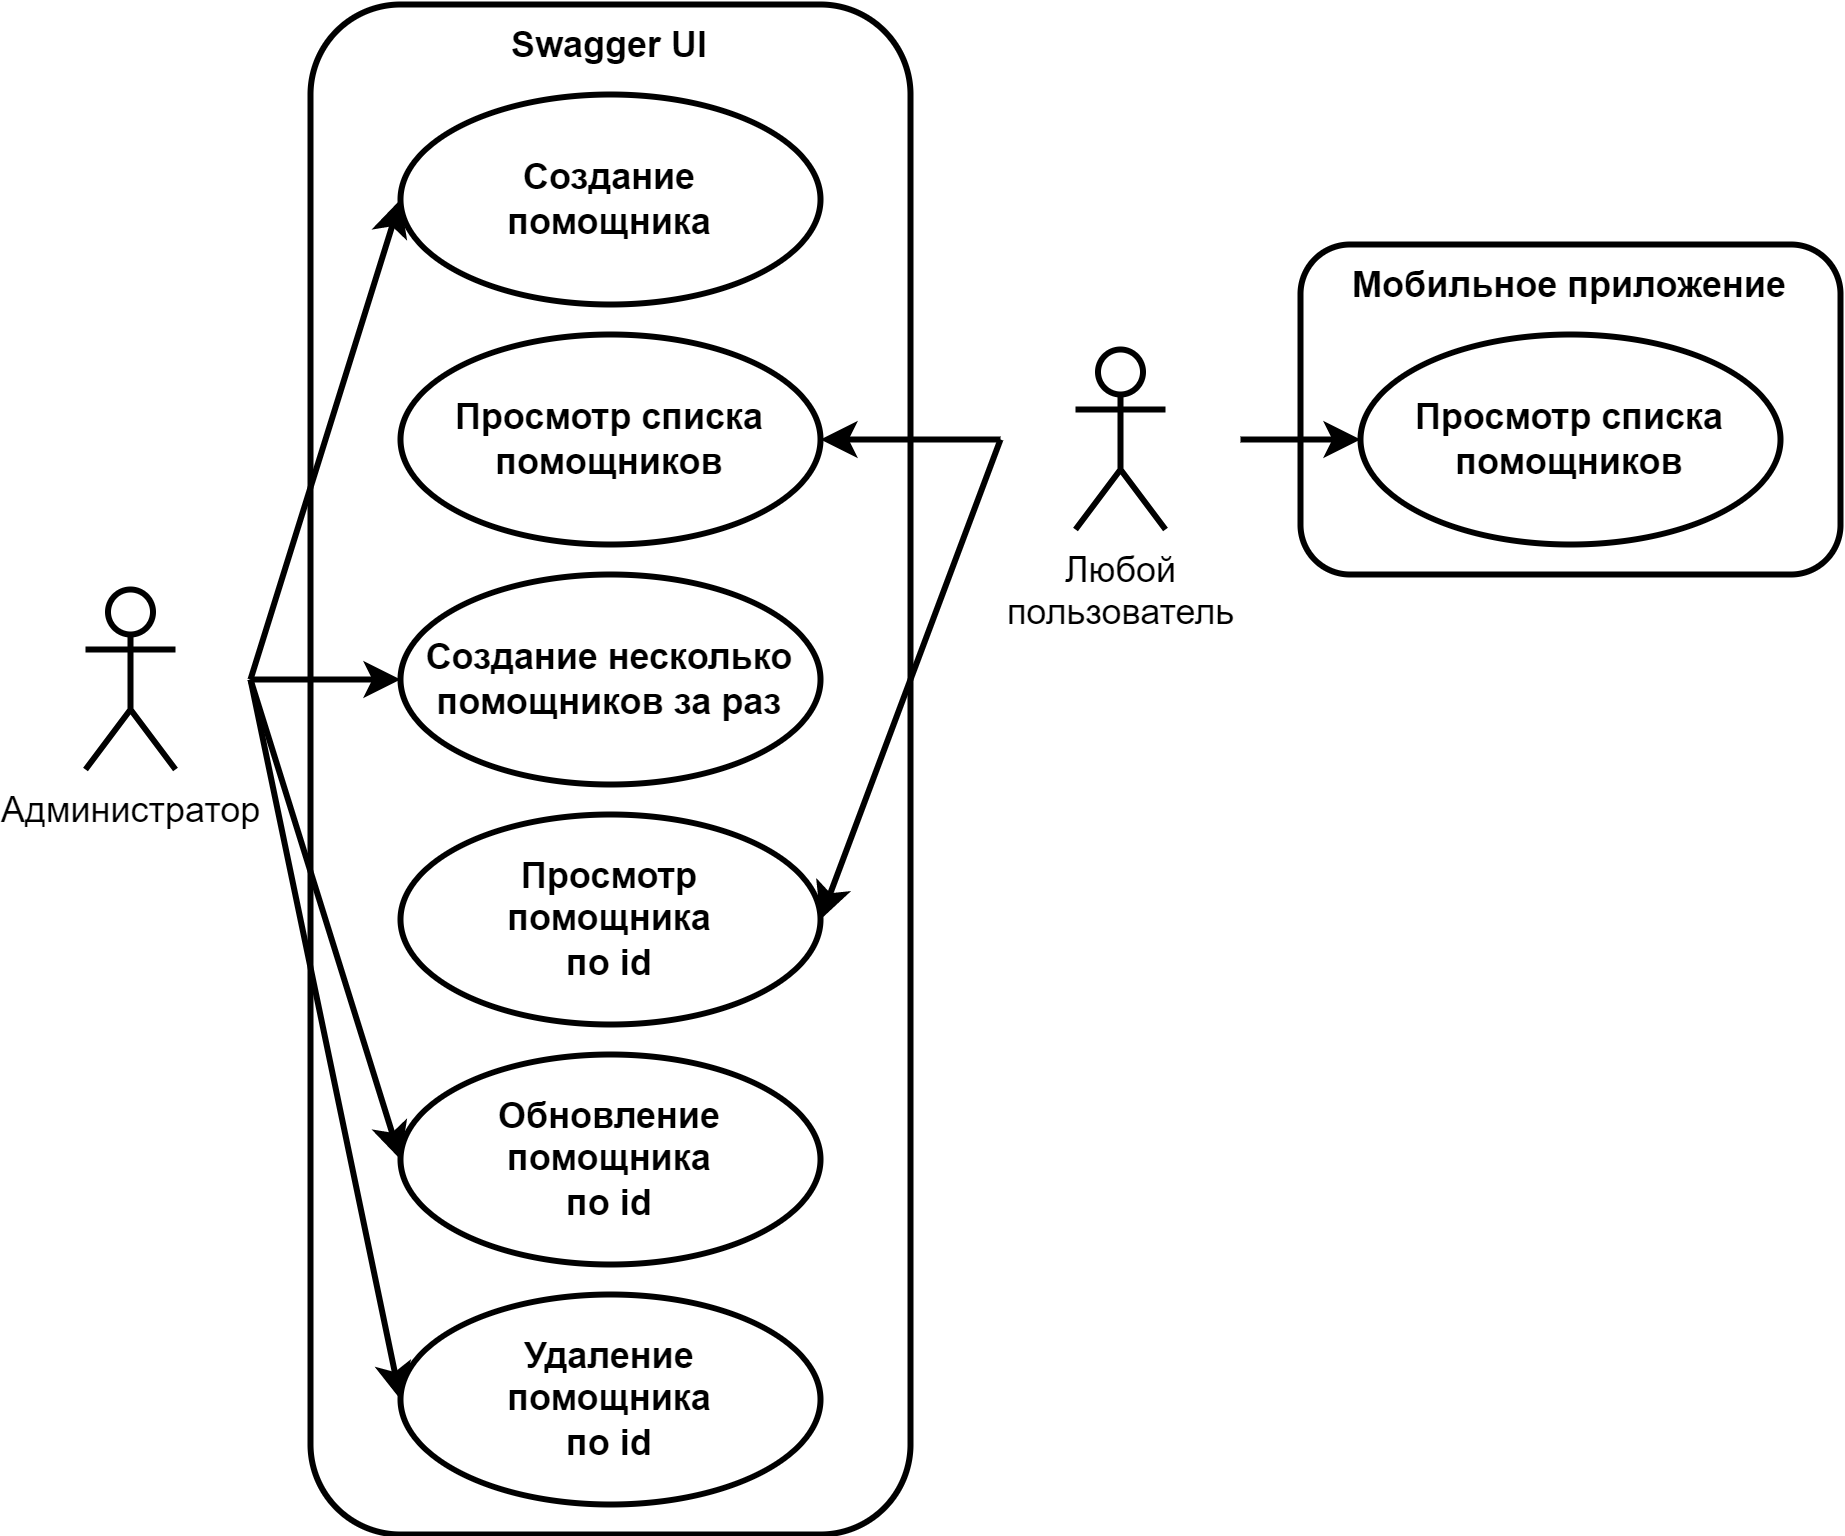
\includegraphics[height=11cm]
    {images/UML/UML_precedent_helpres.png}

    \caption{Диаграмма прецедентов для манипуляции с помощниками}

    \label{fig:UML_precedent_helpres}
\end{figure}

% = = = = = = = =

\subparagraph{Прецедент <<Создание статьи>>} \hspace{0pt}

\underline{Назначение}: создать статью для сайта.

\underline{Исполнители}: администратор, браузер.

\underline{Эндпоинт}: POST /api/v1/articles.

\underline{Предусловие}: у пользователя есть токен доступа и роль admin.

\underline{Основной поток событий}: HTTP статус 201 (Created) - администратор создал статью для сайта в БД. 

\underline{Альтернативный поток событий}:
HTTP статус 500 (Internal Server Error) - что-то пошло не так на сервере.

Диаграмма прецедентов изображены на рис.~\ref{fig:UML_precedent_articles}.

% = = = = = = = =

\subparagraph{Прецедент <<Просмотр списка статей>>} \hspace{0pt}

\underline{Назначение}: просмотр списка статей для сайта.

\underline{Исполнители}: мобильный клиент, браузер.

\underline{Эндпоинт}: GET /api/v1/articles.

% \underline{Предусловие}: 

\underline{Основной поток событий}: HTTP статус 200 (OK) - пользователь получил список статей. 

\underline{Альтернативный поток событий}:
HTTP статус 500 (Internal Server Error) - что-то пошло не так на сервере.

Диаграмма прецедентов изображены на рис.~\ref{fig:UML_precedent_articles}.

% = = = = = = = =

\subparagraph{Прецедент <<Просмотр статьи по urlSegment>>} \hspace{0pt}

\underline{Назначение}: просмотр данных статьи.

\underline{Исполнители}: мобильный клиент, браузер.

\underline{Эндпоинт}: GET /api/v1/articles/:urlSegment.

% \underline{Предусловие}: 

\underline{Основной поток событий}: HTTP статус 200 (OK) - пользователь получил статью по urlSegment. 

\underline{Альтернативный поток событий}:

\begin{itemize}
    \item HTTP статус 404 (Not Found) - данные о статье urlSegment не найдены;
    \item HTTP статус 500 (Internal Server Error) - что-то пошло не так на сервере.
\end{itemize}

Диаграмма прецедентов изображены на рис.~\ref{fig:UML_precedent_articles}.

% = = = = = = = =

\subparagraph{Прецедент <<Обновление статью по uuid>>} \hspace{0pt}

\underline{Назначение}: обновить данные о стаье по uuid.

\underline{Исполнители}: администратор, браузер.

\underline{Эндпоинт}: PATCH /api/v1/articles/:uuid.

\underline{Предусловие}: у пользователя есть токен доступа и роль admin.

\underline{Основной поток событий}: HTTP статус 200 (OK) - администратор обновил данные о статье по uuid. 

\underline{Альтернативный поток событий}:

\begin{itemize}
    \item HTTP статус 404 (Not Found) - данные о статье по uuid не найдены;
    \item HTTP статус 500 (Internal Server Error) - что-то пошло не так на сервере.
\end{itemize}

Диаграмма прецедентов изображены на рис.~\ref{fig:UML_precedent_articles}.

% = = = = = = = =

\subparagraph{Прецедент <<Удаление статьи по id>>} \hspace{0pt}

\underline{Назначение}: удалить данные о статье по id.

\underline{Исполнители}: администратор, браузер.

\underline{Эндпоинт}: DELETE /api/v1/articles/:uuid.

\underline{Предусловие}: у пользователя есть токен доступа и роль admin.

\underline{Основной поток событий}: HTTP статус 200 (OK) - администратор удалил данные о статье по uuid. 

\underline{Альтернативный поток событий}:

\begin{itemize}
    \item HTTP статус 404 (Not Found) - данные о статье по uuid не найдены;
    \item HTTP статус 500 (Internal Server Error) - что-то пошло не так на сервере.
\end{itemize}

Диаграмма прецедентов изображены на рис.~\ref{fig:UML_precedent_articles}.

% = = = = = = = =

\begin{figure}[!p]
    \centering

    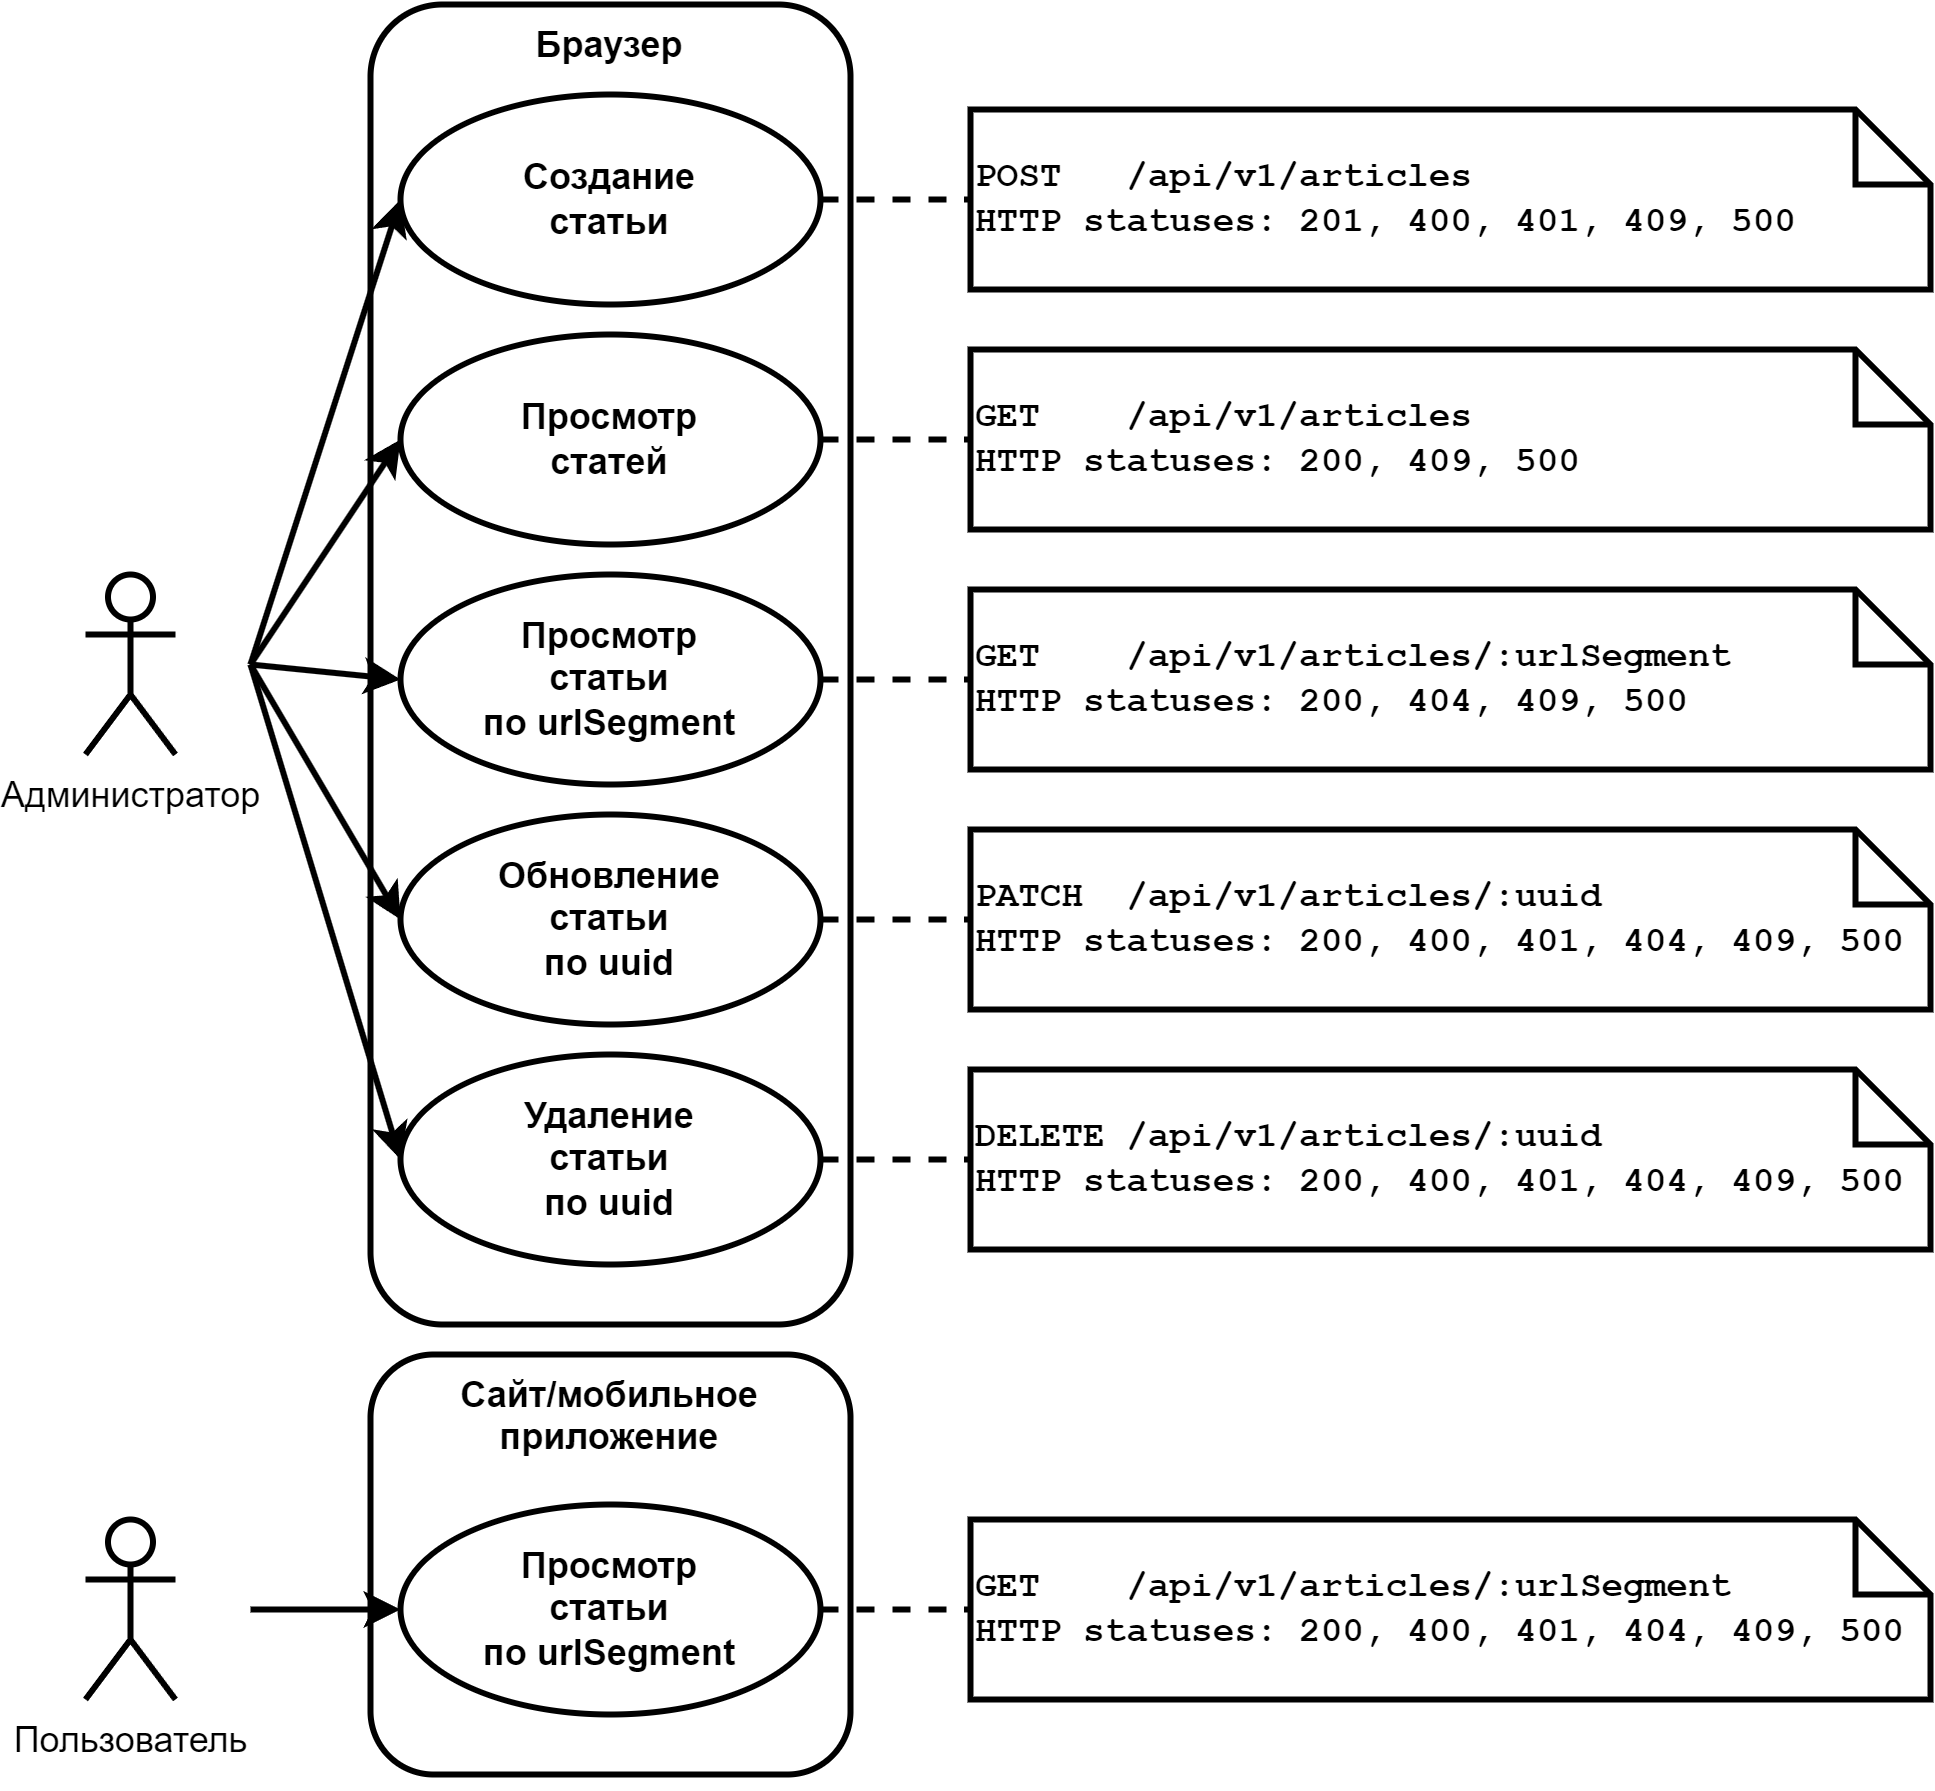
\includegraphics[height=11cm]
    {images/UML/UML_precedent_articles.png}

    \caption{Диаграмма прецедентов для манипуляции со статьями}

    \label{fig:UML_precedent_articles}
\end{figure}

% = = = = = = = =

% \subparagraph{Прецедент <<Просмотр пользователей>>} \hspace{0pt}

% \underline{Назначение}: просмотр списка пользователей.

% \underline{Исполнители}: браузер.

% \underline{Эндпоинт}: GET /api/v1/users.

% \underline{Предусловие}: у пользователя есть токен доступа и роль admin.

% \underline{Основной поток событий}: HTTP статус 200 (OK) - администратор получил список пользователей. 

% \underline{Альтернативный поток событий}:
% HTTP статус 500 (Internal Server Error) - что-то пошло не так на сервере.

% Диаграмма прецедентов изображены на рис.~\ref{fig:UML_precedent_users}.

% = = = = = = = =

% \subparagraph{Прецедент <<Просмотр пользователя по id>>} \hspace{0pt}

% \underline{Назначение}: просмотр данных статьи.

% \underline{Исполнители}: браузер.

% \underline{Эндпоинт}: GET /api/v1/users/:id.

% \underline{Предусловие}: у пользователя есть токен доступа и роль admin.

% \underline{Основной поток событий}: HTTP статус 200 (OK) - администратор получил данные пользователя по id. 

% \underline{Альтернативный поток событий}:

% \begin{itemize}
%     \item HTTP статус 404 (Not Found) - данные о пользователе по id не найдены;
%     \item HTTP статус 500 (Internal Server Error) - что-то пошло не так на сервере.
% \end{itemize}

% Диаграмма прецедентов изображены на рис.~\ref{fig:UML_precedent_users}.

% = = = = = = = =

% \subparagraph{Прецедент <<Блокировка пользователя>>} \hspace{0pt}

% \underline{Назначение}: блокировка пользователя.

% \underline{Исполнители}: браузер.

% \underline{Эндпоинт}: PATCH /api/v1/users/:id/ban.

% \underline{Предусловие}: у пользователя есть токен доступа и роль admin.

% \underline{Основной поток событий}: HTTP статус 200 (OK) - администратор заблокировал пользователя по id. 

% \underline{Альтернативный поток событий}:

% \begin{itemize}
%     \item HTTP статус 404 (Not Found) - пользователь по id не найден;
%     \item HTTP статус 500 (Internal Server Error) - что-то пошло не так на сервере.
% \end{itemize}

% Диаграмма прецедентов изображены на рис.~\ref{fig:UML_precedent_users}.

% = = = = = = = =

% \subparagraph{Прецедент <<Разблокировка пользователя>>} \hspace{0pt}

% \underline{Назначение}: разблокировка пользователя.

% \underline{Исполнители}: браузер.

% \underline{Эндпоинт}: PATCH /api/v1/users/:id/unban.

% \underline{Предусловие}: у пользователя есть токен доступа и роль admin.

% \underline{Основной поток событий}: HTTP статус 200 (OK) - администратор разблокировал пользователя по id. 

% \underline{Альтернативный поток событий}:

% \begin{itemize}
%     \item HTTP статус 404 (Not Found) - пользователь по id не найден;
%     \item HTTP статус 500 (Internal Server Error) - что-то пошло не так на сервере.
% \end{itemize}

% Диаграмма прецедентов изображены на рис.~\ref{fig:UML_precedent_users}.

% = = = = = = = =

% \begin{figure}[!htb]
%     \centering

%     \includegraphics[width=12cm]
%     {images/UML/UML_precedent_users.png}

%     \caption{Диаграмма прецедентов для манипуляции с пользователями}

%     \label{fig:UML_precedent_users}
% \end{figure}

% = = = = = = = =
